% --
% Experiments

\chapter{Experiments}\label{sec:exp}
All experiments performed on the speech command datasets with their obtained results are presented in this chapter.
The speech command datasets are described and analyzed in detail.
Samples from those datasets with their feature extracted representation are shown and the quality and diversity of the recordings is discussed.
The experiments were run on the neural network architectures presented in \rsec{nn_arch}.
In detail the experiments include the feature selection of Mel Frequency Cepstral Coefficients (MFCC) evaluated on Convolutional Neural Network (CNN) architectures, to observe the impact of feature reduction and a frame-based normalization.
Further the transfer of weights from trained Generative Adversarial Neural Networks (GAN) to CNN networks is evaluated.
The performance of a Wavenet architecture operating on raw audio samples is examined.

% dataset
% --
% dataset

\section{Dataset}\label{sec:exp_dataset}
This thesis uses two datasets, one is the second version of the speech commands dataset \cite{Warden2018} and the other is self made consisting of only 5 labels (speech commands) that are especially valuable for movement in video games.
The self made dataset is referred to as \enquote{my dataset} and is used as additional evaluation set.
The training, validation, and testing of the neural network architectures performs on the speech commands dataset.
Both datasets consists of raw waveform files in the \texttt{.wav} format without any feature extraction done beforehand.
As already mentioned in \rsec{prev_kws_benchmark}, the direct comparisons between different neural network approaches is difficult, if the feature extraction is left alone to the user.
Some datasets provide feature extraction beforehand so that the comparability of individual neural network architectures performances is not influenced on it.
The speech commands dataset does not explicitly separate each \texttt{.wav} file into train, test, and validation sets, but provides file lists that refer to distinct waveform files that should be used for testing and validation. 
That means, when the same test and validation sets are used in different research projects, it provides means for comparison to the individual researchers.


% --
% speech commands dataset

\subsection{Speech Commands Dataset}\label{sec:exp_dataset_speech_cmd}
The speech command dataset \cite{Warden2018} consists of \SI{1}{\second} speech recordings, done by over thousands of individual speakers and exists in two versions (\texttt{v0.01} and \texttt{v0.02}).
The first version was published in 2017 with a total number of 30 keywords.
In 2018 the second version extended the first version with 5 additional keywords \{\enquote{backward}, \enquote{forward}, \enquote{follow}, \enquote{learn}, \enquote{visual}\}.
Further, more class examples were added and a better quality check was implemented in order to remove poor quality recordings.

In this thesis, the experiments are solely performed on the second version \texttt{v0.02} of the dataset with hard-facts listed in \rtab{exp_dataset_hard_facts}.
\begin{table}[ht!]
\begin{center}
\caption{Hard facts of the speech commands dataset \texttt{v0.02}.}
\begin{tabular}{ M{5cm}  M{2cm} }
\toprule
%\textbf{label} & \textbf{train} \\
%\midrule
Total number of key words & 35\\
Total number of examples & 105886\\
Total number of speakers & 2618\\
\midrule
%Number of core key words & 20\\
%Number of auxiliary key words & 15\\
Recording duration & 0.4 - \SI{1}{\second}\\
Channels & Mono\\
Bit depth of audio files & \SI{32}{\bit}\\
Sampling frequency & \SI{16}{\kilo\hertz}\\
\bottomrule
\label{tab:exp_dataset_hard_facts}
\end{tabular}
\end{center}
\end{table}
\FloatBarrier
\noindent


All available speech command keywords with their separation in training, test, and validation set are shown in \rtab{exp_dataset_all_labels} located in the appendix.
Some keywords have a significantly higher number of examples per class than others.
This inconsistency of examples per classes emerged from the recording settings, as described in \cite{Warden2018}, where the main keywords were recorded with a higher number of examples from the same speaker.
For instance, the same speaker produces five examples of \enquote{go} and two of \enquote{marvin}.
This makes the keywords separable into so called \emph{core keywords} and \emph{auxiliary keywords}.
The core keywords are the main classification objective and each core keyword should correspond to one individual class label.
Therefore the core keywords have the higher count of samples with about 3700 to 4000 examples each.
In detail the core keywords are \{\enquote{yes}, \enquote{no}, \enquote{up}, \enquote{down}, \enquote{left}, \enquote{right}, \enquote{on}, \enquote{off}, \enquote{stop}, \enquote{go}, \enquote{zero}, \enquote{one}, ..., \enquote{nine} \}.

The auxiliary keywords have the purpose to disturb the classification of the core keywords.
Therefore the auxiliary keywords should be labeled separately with one single class label.
In many papers those auxiliary keywords are labeled as \enquote{unknown}.
In this thesis, the label \enquote{\_mixed} presents a mixture of all auxiliary keywords and the core keywords that were not used for classification.
The \enquote{\_mixed} keywords represent all unknown words that an user might speak and are therefore a very important element in the KWS task for the identification of words that are not in the class dictionary.
Note that the \enquote{\_mixed} label makes the classification task much more challenging because the network has to be more accurate in modeling each core keywords against the other core keywords and additionally to the auxiliary keywords.
In the creation of the examples for the \enquote{\_mixed} label, it is preferable to have an equal number of examples per individual auxiliary keyword and unused core keywords.
This was done by placing all unused core keywords and auxiliary words into a separate folder and reading them into an ordered list.
This list is ordered such that one example per keyword is placed consecutively to the next and repeated until all examples were added.
The auxiliary keyword examples picked for training are referenced by the entries of the ordered list, starting from index 0 to the number of training examples per class.

To examine the recorded examples from the speech command dataset, \rfig{exp_dataset_speech_cmd_wav_grid} shows one example from all available speech commands and presents them in raw audio format, where vertical lines indicate the onset detection and end of a \SI{500}{\milli\second} window.
\begin{figure}[!ht]
  \centering
    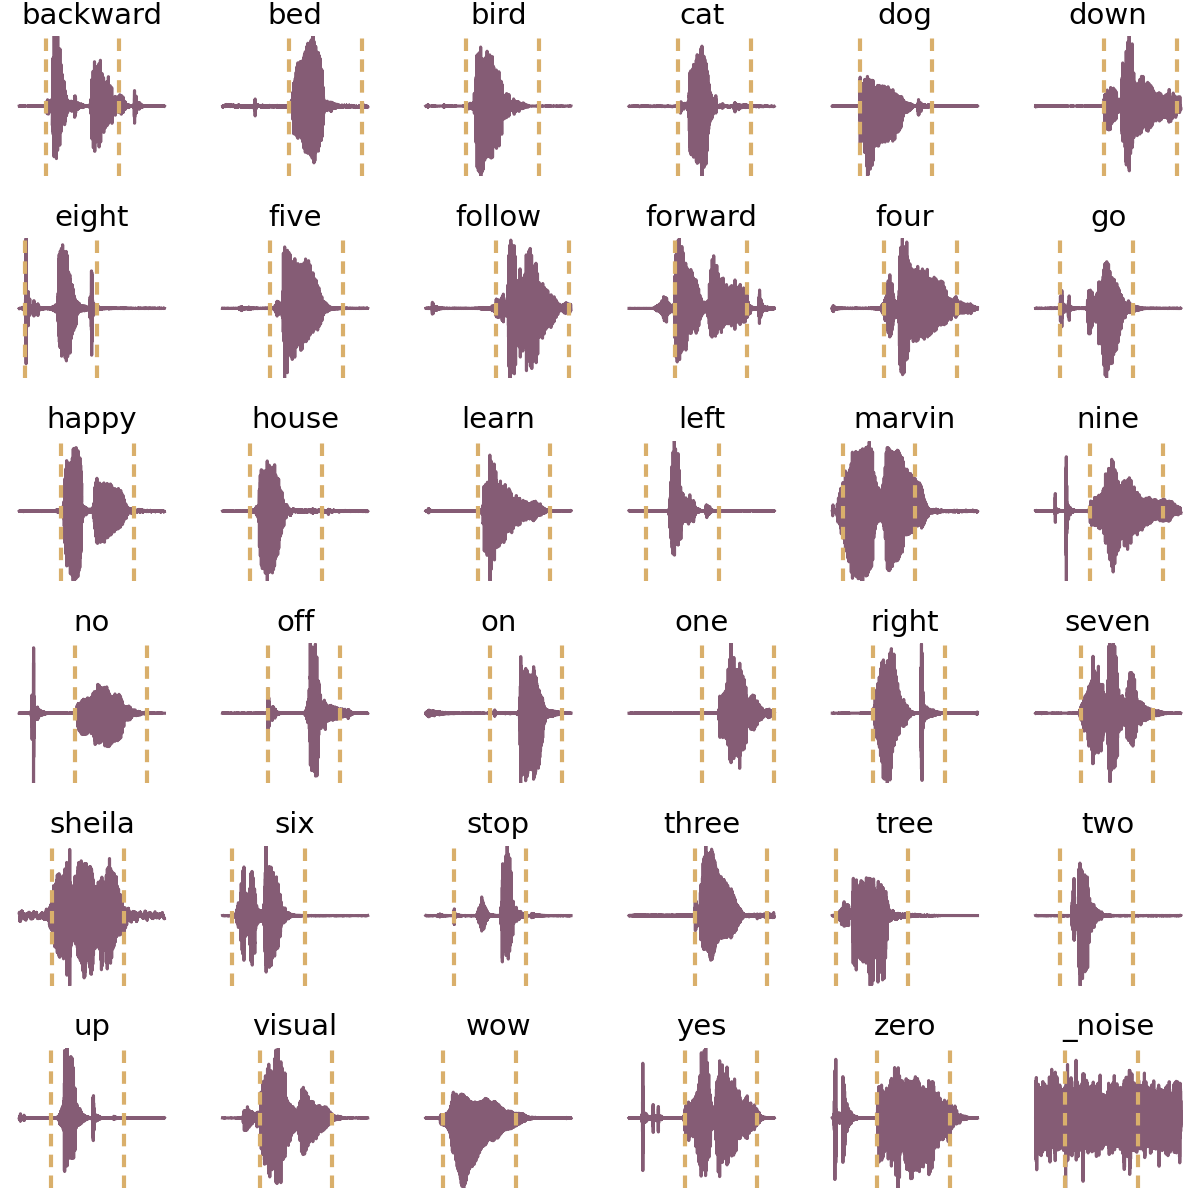
\includegraphics[width=0.65\textwidth]{./5_exp/figs/exp_dataset_speech_cmd_wav_grid.png}
  \caption{One random sample of each individual speech command in the speech command dataset presented in normalized audio waveform.}
  \label{fig:exp_dataset_speech_cmd_wav_grid}
\end{figure}
\FloatBarrier
\noindent


% --
% statistics

\subsubsection{Observations of all available Examples in the Dataset}
Two histograms were created to observe the quality of all recorded files in the dataset.
Those histograms present an energy measure and a count of the sample length for each file.
The energy of a recorded file provides information about a recordings amplification setting and is an indicator for too silent or too loud (overdrive distortions) samples.
In the first version of the speech command dataset, namely \texttt{v0.01}, the silent files were a problem.
This had been fixed in the second version by rejecting those files.
Therefore, the version \texttt{v0.01} is slightly more unclean than \texttt{v0.02}.
The energy value $e \in \R$ can be computed by
\begin{equation}\label{eq:exp_dataset_energy}
  e = \frac{1}{n} \left( \bm{x}^T \bm{x} \right),
\end{equation}
where $\bm{x} \in \R^n$ represents a single recorded file with a total number of $n$ samples.
The division through the sample length $n$ of each individual audio recording is required because not every file has a duration of \SI{1}{\second} (16000 samples).
For an unknown reason, many of the recordings consist of less than 16000 samples, which would be problematic if the sample length is too short to fully capture a keyword.
So the minimum duration of all examples was determined and found to last about \SI{0.4}{\second}.
This however, is adequate for words like \enquote{go}, where the reduced samples length often shows up.
\rfig{exp_dataset_hist} shows the mentioned histograms of all available examples in the dataset.
\begin{figure}[!ht]
  \centering
    \subfigure[energy measure]{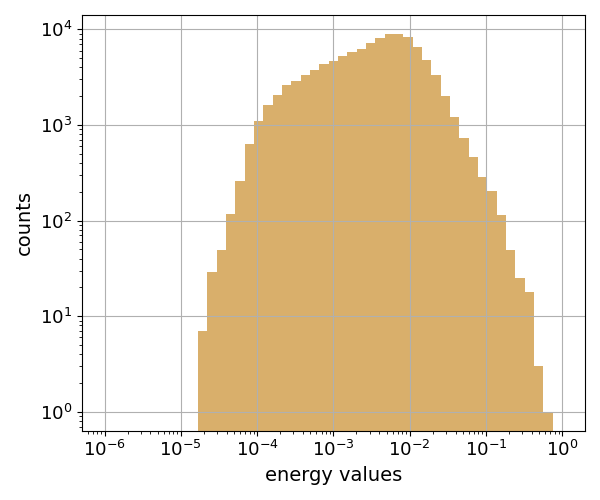
\includegraphics[width=0.42\textwidth]{./5_exp/figs/exp_dataset_hist_energy_overall.png}}
    \qquad
    \subfigure[count of sample length]{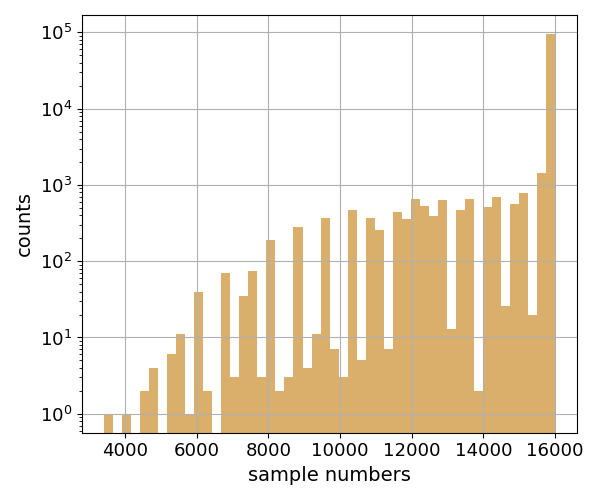
\includegraphics[width=0.42\textwidth]{./5_exp/figs/exp_dataset_hist_sample_overall.png}}
  \caption{Histograms of all available examples in the speech commands dataset \texttt{v0.02}, where one histogram shows an energy measure in log-log scale and the other a count of the sample length in log scale.}
  \label{fig:exp_dataset_hist}
\end{figure}
\FloatBarrier
\noindent
The histogram of the energy measure has one main lobe, which implies that there are no clusters of extremely silent or loud files.
For comparison, if silent files were extracted from the given background files, the energy of some of those would be in a range of $10^{-7} \dots 10^{-6}$ indicating that those files are too silent.
The sample length histogram shows that most of the files consist of 16000 samples but many others have a smaller number of samples. 
This is relevant and has to be considered in the pre-processing of audio files because inputs to neural networks often have to be prepared to fixed size inputs if no sequential neural networks, such as RNNs, are used.


% --
% recording quality

\subsubsection{Recording Quality and Personal Experience}
The examples of the speech commands dataset \cite{Warden2018} were not recorded by professionals with high-end recording equipment.
In fact the recordings had been done in an amateur kind of fashion so that the dataset is more suited to realistic environments intended for user applications.
This is also noted in the paper \cite{Warden2018}:
\begin{quote}
...This meant that the use of studio-captured samples seemed unrealistic, since that audio would lack background noise, would be captured with high-quality microphones, and in a formal setting. 
Successful models would need to cope with noisy environments, poor quality recording equipment, and people talking in a natural, chatty way...
\end{quote}
The recording devices of the speakers, who contributed examples to the dataset, were in most cases consumer microphones, as for instance, embedded microphones in laptops or mobile phones.

The conclusions drawn from listening to the examples in the dataset are as follows:
\begin{itemize}
  \item The quality of the examples in the dataset are ranging from excellent and perfectly recognizable to very poor, noisy, unrecognizable, and cut off. Although most of the examples are provided with sufficient quality.
  \item Different accents had been perceived, which suggests that people from several nationalities were involved.
  However, the bias was laid on American English, as noted in the paper.
  \item No children speakers had been found.
\end{itemize}
Due to data privacy issues the information of individual speakers is not displayed.
Therefore, it is not clear whether the dataset consists of an equal amount of male and female speakers and whether there are any children speakers included.
The last would be especially interesting for a video games intended for children.

In many recordings the background noise is imminent, such as traffic noise, chattering people, office sounds, and many more.
A quality check of the recorded files in the dataset had been done beforehand to ensure that poor quality examples are rejected.
Nevertheless, there are still some existing flaws, such as extremely loud or silent recordings, examples with inconsistent sample numbers, recordings that include too much noise or in the worst case noise only (very rarely), and cut off signals capturing only half of a word.
Those quality issues in the dataset can for most cases be neglected or fixed, such as inconsistent sample numbers. 
Other more problematic cases, like noise-only examples, should ideally be removed.
But since their occurrence is very rare it is not worth the effort.
Besides, it is usually not a problem for neural networks to cope with noisy datasets.
In many cases it is favorable when a dataset contains many noisy samples so that neural networks can learn invariance against noise, loudness differences, and other nuisances during training.
Moreover, if the training dataset is sufficiently large, and the test and validation sets do not contain very poor examples, there should be no problem in the training and evaluation of different models.
Finally, it has to be acknowledged that the dataset is published under the creative common license, hence it is freely available to everyone, which is simply fabulous.


% --
% dataset structure

\subsubsection{Dataset Structure}\label{sec:exp_dataset_structure}
The speech command examples are stored in separate folders named after each individual keyword.
The folder named as \texttt{\_background\_noise\_} contains six different background noise files, such as \texttt{white\_noise.wav} or \texttt{doing\_the\_dishes.wav}, with a duration of more than one minute each and altogether summing up to a duration of about \SI{400}{s}.
To extract noise examples from those files with a sufficient number of examples of over 3500, those noise files have to be extracted by a striding window of \SI{1}{\second} length shifted by \SI{0.110}{\second}.
The noise examples were assigned to the label \enquote{\_noise}.

Each waveform file from the keyword folders is named by an 8-digit hexadecimal hash code for the speaker identification and followed by the utterance number, for instance \texttt{3b4f8f24\_nohash\_0.wav}.
With the speaker identification code known it is possible to distinguish between different speakers.
However, as mentioned above, no further information about the speakers is provided due to data privacy issues.

Moreover, the dataset contains a testing file list called \texttt{testing\_list.txt} and a validation file list \texttt{validation\_list.txt}, where each row entry in the text file refers to a file in the dataset, as for example \texttt{right/bb05582b\_nohash\_3.wav}.
Those file lists should ensure the comparability between different neural network approaches from individual researchers.
The testing and validation file lists are applied in this thesis and the separation into sets are shown in \rtab{exp_dataset_all_labels}.


% --
% extracted examples

\subsubsection{Samples from the Feature Extraction}
The feature extracted data examples are stored to separate files before using them for training.
This has the practicability that features do not have to be extracted each time a new training instance of a neural network is performed.
Samples from the extracted MFCCs with frame-based normalization, as explained in \rsec{signal_mfcc}, are shown in \rfig{exp_dataset_speech_cmd_mfcc}.
\begin{figure}[!ht]
  \centering
    \subfigure[left]{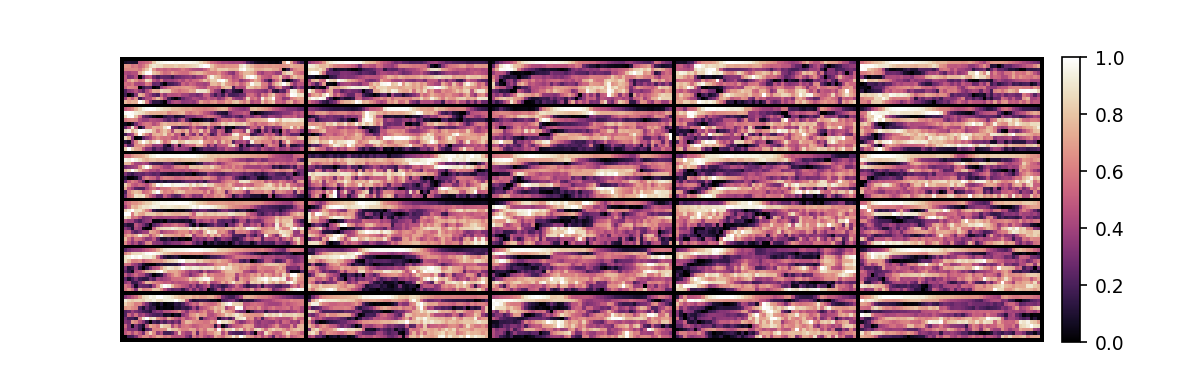
\includegraphics[width=0.48\textwidth]{./5_exp/figs/exp_dataset_speech_cmd_mfcc_left.png}}
    \subfigure[right]{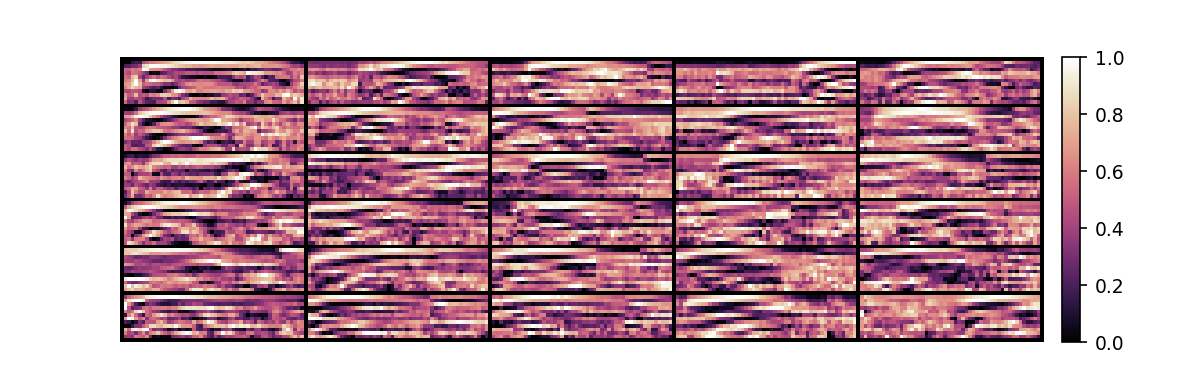
\includegraphics[width=0.48\textwidth]{./5_exp/figs/exp_dataset_speech_cmd_mfcc_right.png}}
    \subfigure[up]{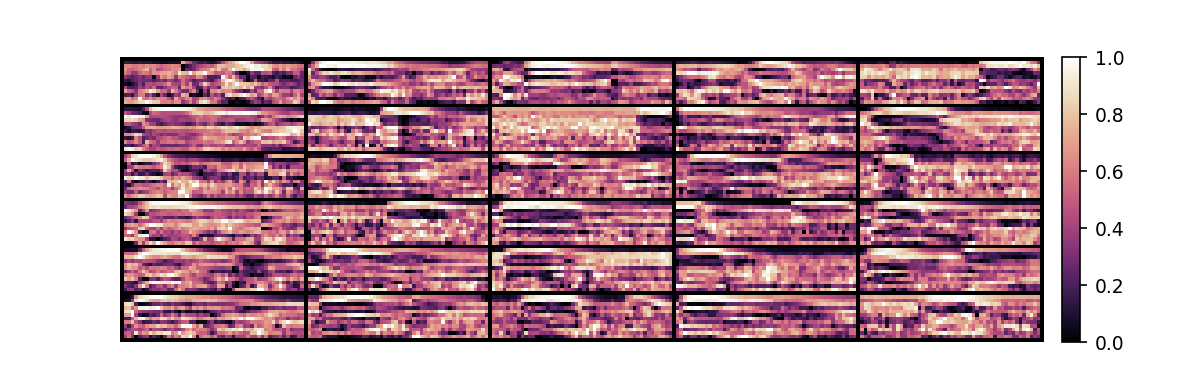
\includegraphics[width=0.48\textwidth]{./5_exp/figs/exp_dataset_speech_cmd_mfcc_up.png}}
    \subfigure[down]{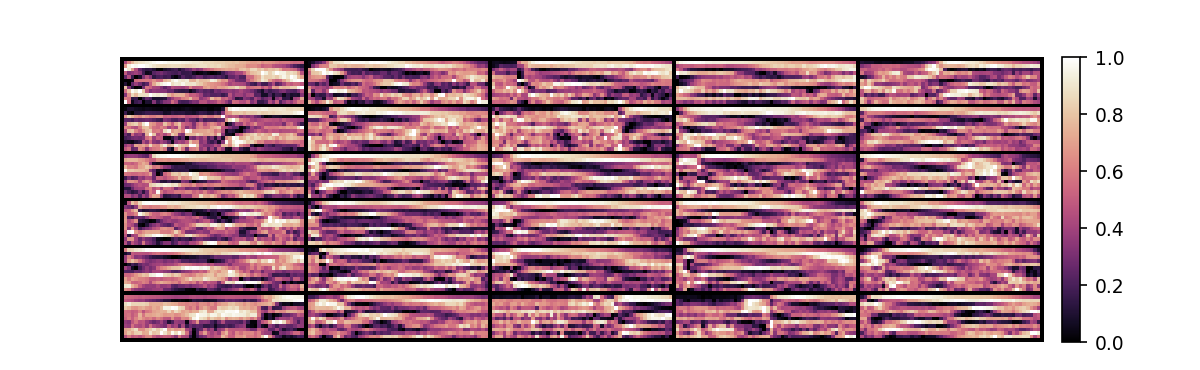
\includegraphics[width=0.48\textwidth]{./5_exp/figs/exp_dataset_speech_cmd_mfcc_down.png}}
    \subfigure[go]{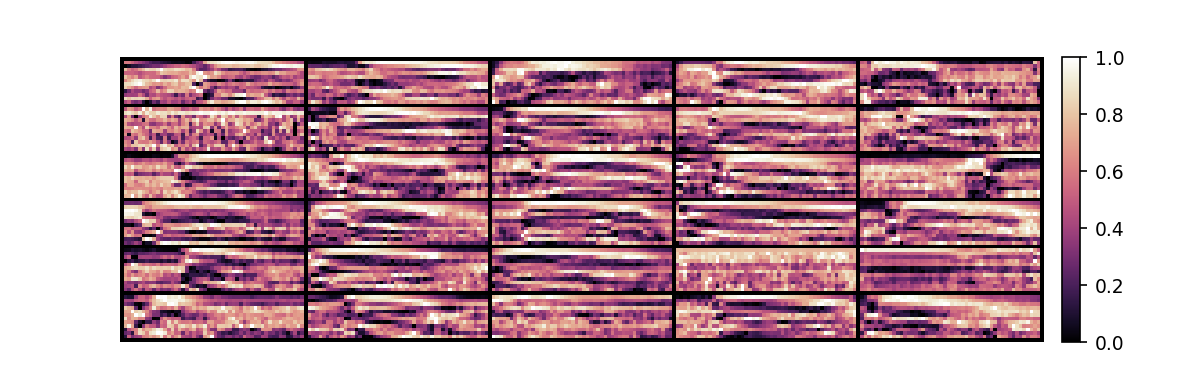
\includegraphics[width=0.48\textwidth]{./5_exp/figs/exp_dataset_speech_cmd_mfcc_go.png}}
  \caption{MFCC extraction of randomly selected 30 samples per class label obtained from the training set of the speech commands dataset \texttt{v0.02}. The corresponding class labels are written below the plots.}
  \label{fig:exp_dataset_speech_cmd_mfcc}
\end{figure}
\FloatBarrier
\noindent


% --
% my dataset

\subsection{My Dataset}\label{sec:exp_dataset_my}
This dataset was created by the author of this thesis and contains five examples for each of the following keywords \{\enquote{left}, \enquote{right}, \enquote{up}, \enquote{down} and \enquote{go}\}.
The datasets purpose is mainly to have an additional test set for evaluating trained models on the authors own voice.
The examples per keyword are spoken with different emphasis and stress on individual phonemes for each keyword.
Also the prolongation of the words are different, for instance, in one example the word is spoken very hasty and in the other it is spoken slowly.
The emphasis and prolongation ensure the diversity of the dataset.
It is relevant to mention that none of the self recorded files were used within the training set so that the neural networks performance is evaluated on unseen data.
All examples of \enquote{my dataset} are illustrated in \rfig{exp_dataset_my_wav_grid} in raw audio format.
\begin{figure}[!ht]
  \centering
    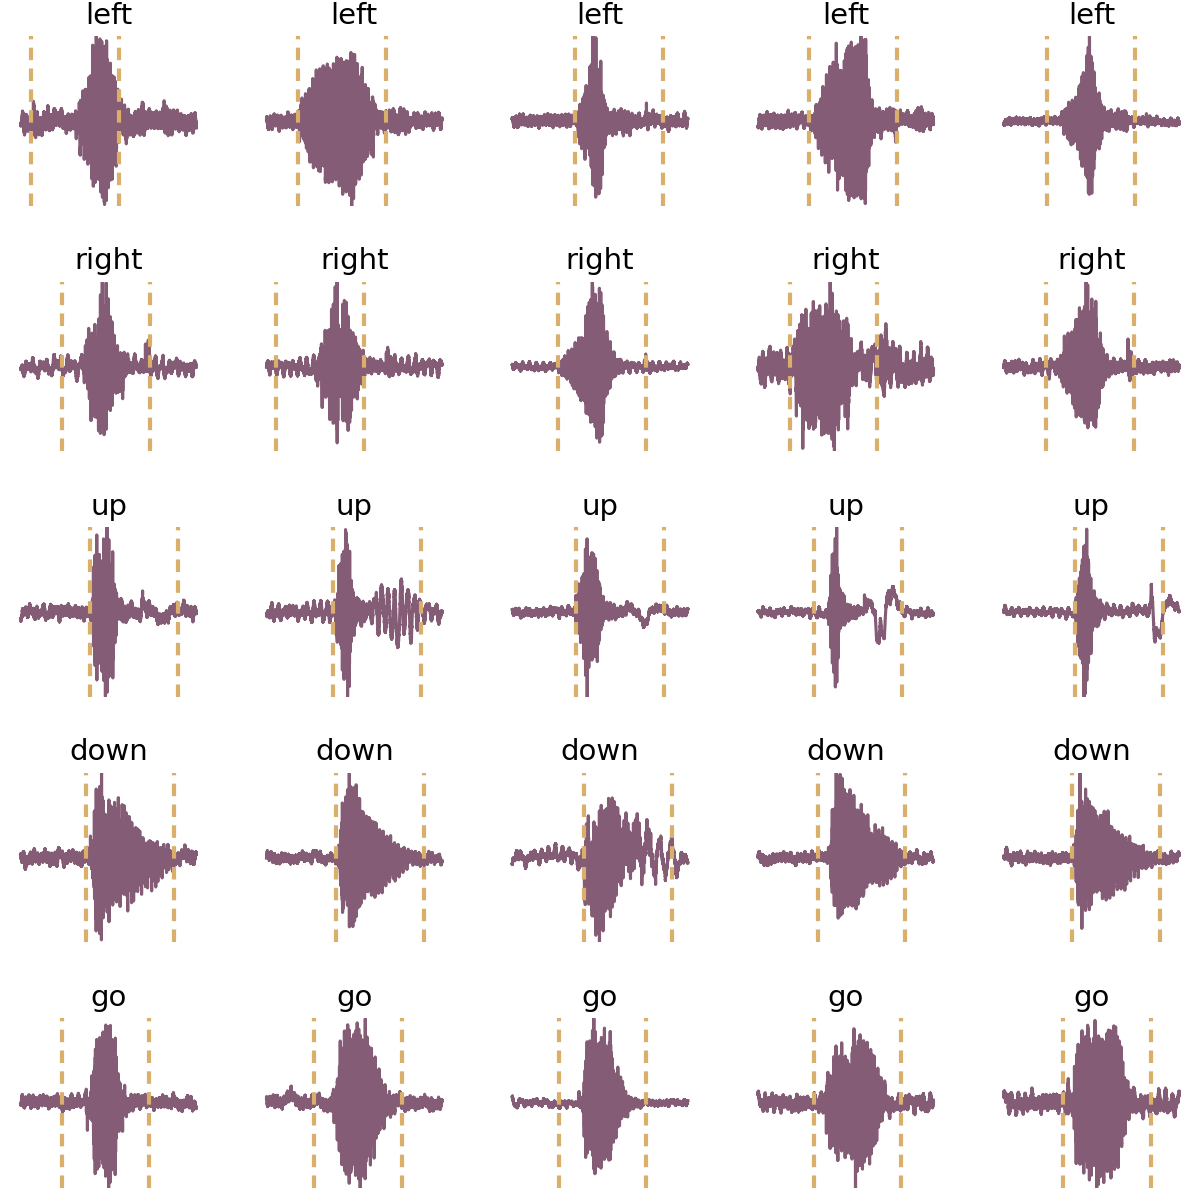
\includegraphics[width=0.6\textwidth]{./5_exp/figs/exp_dataset_my_wav_grid.png}
  \caption{Self recorded files of the \enquote{my dataset} in raw audio format.}
  \label{fig:exp_dataset_my_wav_grid}
\end{figure}
\FloatBarrier
\noindent
The same examples extracted to MFCC features are shown in \rfig{exp_dataset_my_mfcc}.
\begin{figure}[!ht]
  \centering
    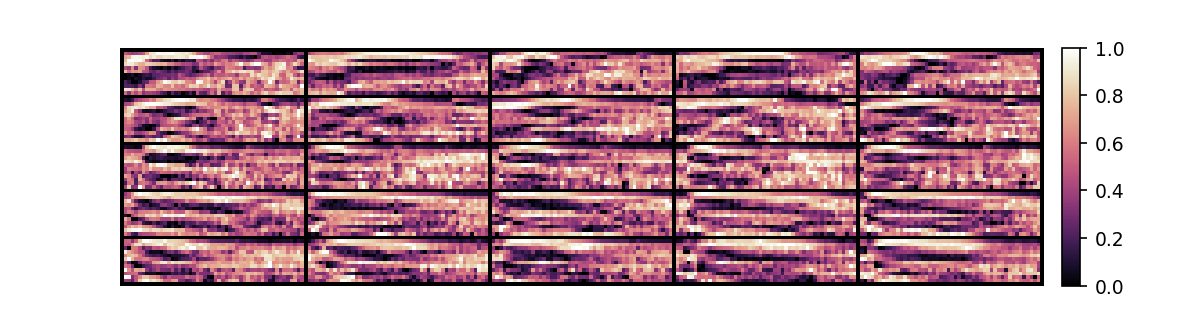
\includegraphics[width=0.65\textwidth]{./5_exp/figs/exp_dataset_my_mfcc.png}
  \caption{All MFCC extracted samples of the \enquote{my dataset} with the same ordering as shown in \rfig{exp_dataset_my_wav_grid}.}
  \label{fig:exp_dataset_my_mfcc}
\end{figure}
\FloatBarrier
\noindent
It turned out that it is a very hard task for neural networks to achieve a \SI{100}{\percent} classification score upon it, despite the fact that all examples correspond to the same speaker.
This is slightly worrying because acoustically each of the examples per word is perfectly distinguishable for humans.
For instance, in the classification of the five examples of \enquote{left} from the \enquote{my dataset}, the trained models may classify 4 examples as \enquote{left} and one as \enquote{right}.
It is difficult to examine why exactly this single example was wrongly classified.


% --
% preparation for neural networks

\subsection{Data Preparation for Neural Networks}\label{sec:exp_data_prep}
The neural network architectures are trained with supervised learning.
This implies that a class label $y_i \in \{0, 1, \dots, L\}$ correspondence to each data example $x_i \in \mathcal{X}$ exists, where $L$ is the total number of classes and $\mathcal{X}$ is the input space of the data example.
The input space for MFCC features is, for example, $\mathcal{X} = \R^{C \times M}$ with $C$ cepstral coefficients and $M$ frames.
Selected examples including their labels form a set $S$, for example for training or testing, which can be written as
\begin{equation}\label{eq:exp_dataset}
  S = \{ (x_i, y_i) \mid i = 0, 1, \dots, n \},
\end{equation}
where $n$ is the total number of examples within this set.
Class labels $y_i$ are usually translated to integer numbers that are referencing to indices in a class dictionary.
For instance, $y_1 = 0$ of example $i=1$ refers to the label \enquote{left} in the dictionary \{0: \enquote{left}, 1: \enquote{right}\}.
It is essential that the enumeration of class labels in the class dictionary starts from zero because they should correspond to the output nodes in the used neural network.

\rsec{signal_mfcc} already showed how to extract MFCC features.
Nevertheless, it is important that each individual $x_i$ for all $i$ has the same dimension $\mathcal{X}$ so that a data preparation for the training of neural networks is possible.
It could happen that the sample numbers of the waveform files are inconsistent, as described in \rsec{exp_dataset_speech_cmd}, and therefore different dimension of individual data examples may be obtained.
To ensure that all $x_i$ have the same dimension, the audio files were adjusted to the same fixed sample length of a duration of \SI{1}{\second} and sampling frequency \SI{16}{\kilo\hertz}.
This was achieved by zero-padding the signals to the desired fixed length of $n = 16000$ samples.
Furthermore, a dither noise was added so that neural networks are not confused when operating on pure zeros that emerge from the data examples.
Additive White Gaussian Noise (AWGN) ensures an appropriate dithering of the data examples by
\begin{equation}\label{eq:exp_dither}
  \bm{x} = \bm{\tilde{x}} + \bm{v}, \quad \bm{v} \sim \mathcal{N}(\mu=0, \sigma=0.5 \cdot \tilde{x}_{quant}),
\end{equation}
where $\bm{v} \in \R^n$ is sampled from the normal distribution $\mathcal{N}$ with standard deviation given by the quantization error $\tilde{x}_{quant} \in \R$, $\bm{\tilde{x}} \in \R^n$ is the zero-padded signal (only if the total sample number is less than 16000).
The quantization error $\tilde{x}_{quant}$ corresponds to the minimum of all absolute values from the samples of $\bm{\tilde{x}}$, except the pure zero entries added through zero-padding.
When the dithering is applied to the signal, the pure zeros are overwritten by the sampled dither noise while at the same time a minimal altering of the original signal is achieved.
This is because the maximum change is in range of a normal distribution of the quantization error from the original recording.

% training details
% --
% training details

\section{Implementation and Experiment Details}\label{sec:exp_details}
The implementation details describe the used software tools in the experiments, such as the programming language and packages for the source code.
The experiment details are separated into training details of the used neural networks and evaluation details of the trained models.
The training details provide the used sets of hyperparameters for the training of the neural networks on the speech commands dataset.
Note that the training details can vary in different experiments.
If they do so, they are usually noted in the description of the corresponding experiment, otherwise the parameters listed are used.
The evaluation details describe how the trained models are evaluated in regards of accuracy performance and noise and shift invariance.


% --
% implementation notes

\subsection{Implementation Notes}\label{sec:exp_details_implementation}
The source code for this thesis was written in \texttt{Python} with version $>3.8$ and tested on a Linux operating system.
Further, the source code is open source available in \cite{KWSGame}.
The operating system might be relevant if someone tries to run the python code on a \enquote{Windows} machine, where unexpected errors might occur (especially regarding path variables).
Note that the project does not explicitly download the speech commands dataset.
A path variable to the downloaded dataset has to be specified in the \texttt{config.yaml} file of the project, where users may also change several other useful parameters.
More information about how to run the project is described in the \texttt{README.txt} file.
The training and implementation of all used neural networks were done with the \texttt{Pytorch} \cite{Pytorch} framework of version $>1.7.0$. 
The feature extraction of MFCCs was self implemented but used already existing and efficient code for signal transformations, such as the STFT or DCT provided by the \texttt{Scipy} package.
All matrix-vector computations were processed with the well known \texttt{Numpy} package or with \texttt{Pytorch}.
Several other \texttt{Python} packages were used within the project but are not named explicitly.
They can be looked up in the open source repository of the project, if requested.


% --
% training details

\subsection{Neural Network Training Details}\label{sec:exp_details_training}
The training details and parameters of the used neural networks can be split into following components: Feature extraction, dataset, training, and pre-training.
The feature extraction parameters provide information about the extraction of MFCC features.
The dataset parameters are specified by the selected labels and the number of examples per labels for training.
The training part lists hyperparameters, such as the learning rate or the batch size.
Furthermore, the pre-training details describe a separate training of GANs to use the obtained weights for transfer learning on an equivalent CNN.


% --
% feature

\subsubsection{Feature Extraction Parameters}
The feature extraction parameters used in order to process MFCCs, are listed in \rtab{exp_details_params_feature}.
Note that some parameters can vary in the experiments.
% --
% feature extraction parameters
\begin{table}[ht!]
\begin{center}
\caption{Parameters for MFCC feature extraction.}
\begin{tabular}{ M{6cm}  M{2cm} M{2cm}}
\toprule
\textbf{Parameter} & \textbf{Value} & \textbf{Varying for experiments} \\
\midrule
Speech signal length & \SI{500}{\milli\second} & - \\
Analytic window size & \SI{25}{\milli\second} & -\\
Hop size & \SI{10}{\milli\second} & -\\
Window Function & Hanning & -\\
\midrule
Number of filter bands & 32 & -\\
Number of cepstral coefficients & 12 & yes\\
Delta features & no & yes \\
Double delta features & no & yes \\
Energy features & no 	& yes \\
Frame based normalization & yes & yes\\
\bottomrule
\label{tab:exp_details_params_feature}
\end{tabular}
\end{center}
\end{table}
\FloatBarrier
\noindent


% --
% dataset

\subsubsection{Dataset Parameters}
The labels for training are selected to the same 12 labels (L12) that were also used in the benchmark models in \rsec{prev_kws_benchmark}.
Therefore, the L12 labels ensure a valid comparison between the performed experiments in this section and the benchmark models.

The maximum number of examples per label for training and evaluation is given by the minimum examples of each selected label in each set.
This is provided by the label \enquote{go} with following amount of examples in the sets: \{train: 2948, test: 425, validation: 350 \} from \rtab{exp_dataset_all_labels}.
Hence, the validation set consists of 350 examples of the label \enquote{go}.
By considering a \SI{10}{\percent} split of both test and validation set, this gives a maximum amount of 3500 examples per label to represent the whole dataset.
Therefore, the number of examples per label should not exceed the value 3500, otherwise the equal amount of examples per label is not provided.
Note that in order to reduce computations in some experiments, the number of examples were reduced to only 500 per label.
\rtab{exp_details_params_dataset} lists the L12 labels and their number of examples per label used for training.
\begin{table}[ht!]
\small
\begin{center}
\caption{Parameters for the dataset extraction.}
\begin{tabular}{ M{7cm}  M{6cm}}
\toprule
\textbf{Parameter} & \textbf{Value} \\
\midrule
class dictionary with 12 labels (L12) & \{\enquote{left},  \enquote{right}, \enquote{up}, \enquote{down}, \enquote{go}, \enquote{stop}, \enquote{yes}, \enquote{no}, \enquote{on}, \enquote{off}, \enquote{\_mixed}, \enquote{\_noise}\}\\
action set used in the video game & \{\enquote{left},  \enquote{right}, \enquote{up}, \enquote{down}, \enquote{go}, \enquote{\_mixed}, \enquote{\_noise}\}\\
\midrule
number of examples per label & 500 or 3500 (whole dataset) \\ 
\bottomrule
\label{tab:exp_details_params_dataset}
\end{tabular}
\end{center}
\vspace{-4mm}
\end{table}
\FloatBarrier
\noindent
Note that the actions set of the deployed video game in \rsec{game} uses only a subset of the L12 labels, namely the set: \{\enquote{left},  \enquote{right}, \enquote{up}, \enquote{down}, \enquote{go}, \enquote{\_mixed}, \enquote{\_noise}\}.
Still the video game operates with the models trained on the L12 labels and thus might increase the chance in confusing keywords.


% --
% training hyperparameters

\subsubsection{Training Hyperparameters}
\rtab{exp_details_params_train} shows the hyperparameters for the training of the used CNNs models, described in \rsec{nn_arch}.
% --
% feature extraction parameters
\begin{table}[ht!]
\begin{center}
\caption{Parameters for training neural networks.}
\begin{tabular}{ M{6cm}  M{2cm} M{2cm}}
\toprule
\textbf{Parameter} & \textbf{Value} & \textbf{Varying for experiments} \\
\midrule
Number of epochs & 1000 & yes\\
Batch size & 32 & -\\
\midrule
Optimizer & Adam & -\\
Learning rate & 0.0001 & -\\
Momentum & 0.9 & -\\
\bottomrule
\label{tab:exp_details_params_train}
\end{tabular}
\end{center}
\vspace{-4mm}
\end{table}
\FloatBarrier
\noindent
From the following experiments, it can be observed that epochs of 2000 yield into small overfitting effects regarding certain models.
This might decrease the accuracy performance if the set of parameters is used at the last epoch and no early stopping mechanism is applied.
The batch size of 32 is selected to a low number because it worked well on the KWS task of speech commands.
Further, the amount of classes is at maximum 12 (L12 labels) and therefore a batch size of 32 would include most of the individual labels.
Note that the hyperparameters for the Wavenet model are described in the corresponding experiment section.


% --
% training parameters

\subsubsection{Pre-Training Details}
The pre-training parameters describe the training of the GANs with their models presented in \rsec{nn_arch_adv}.
The hyperparameters listed in \rtab{exp_details_params_pre_train}, are the same as for usual training but the Discriminator and Generator network can have each different values.
\begin{table}[ht!]
\begin{center}
\caption{Parameters for adversarial pre-training of a Generator and a Discriminator network.}
\begin{tabular}{ M{6cm}  M{2cm} M{2cm}}
\toprule
\textbf{Parameter} & \textbf{Value} & \textbf{Varying for experiments} \\
\midrule
Number of epochs & 1000 & yes\\
Batch size & 32 & -\\
\midrule
Optimizer & Adam & -\\
Learning rate Generator & 0.0001 & -\\
Learning rate Discriminator & 0.0001 & -\\
Momentum Generator & 0.9 & -\\
Momentum Discriminator & 0.9 & -\\
\bottomrule
\label{tab:exp_details_params_pre_train}
\end{tabular}
\end{center}
\vspace{-4mm}
\end{table}
\FloatBarrier
\noindent
The selection of the epochs is important, as it was already pointed out in \rsec{nn_adv}.


% --
% evaluation details

\subsection{Evaluation Details}\label{sec:exp_details_tb}
The main evaluation score of the trained models is the accuracy performance on the test sets.
The accuracy is obtained by counting all correct classifications and dividing it by the number of classified samples $n$.
A score function $c(\hat{y}_i, y_i)$ for the accuracy can be defined by
\begin{equation}
  c(\hat{y}_i, y_i) = 
  \begin{cases}
    1, & \text{if } \hat{y}_i = y_i\\
    0, & \text{otherwise} 
  \end{cases},
\end{equation}
where $\hat{y}_i \in \mathcal{L} = \{0, 1, \dots, L\} $ is the predicted label and $y_i \in \mathcal{L}$ the actual label of the sample $i$ with a total number of class labels $L$.
The accuracy $a \in [0, 1]$ therefore formulates as
\begin{equation}
  a = \frac{1}{n} \sum_{i=0}^n c(\hat{y}_i, y_i).
\end{equation}
Another, more unconventional evaluation technique, is the evaluation upon noise and shift invariance of dedicated test signals.
For this, one example of each class label was taken from the self recorded files of the \enquote{my dataset} and used as test signal.
The length of those audio files is cut such that by applying a fixed input frame of \SI{500}{\milli\second} both end positions consist of at least the half of the audio file's information.
This is especially relevant to the shift invariance test.
The evaluation results are plotted in figures of correct classification upon noise level and shift index changes of the test signals.
Note that the noise and shift invariance are tested on only 5 test signals.
Therefore, they are not a reliable measure for the trained models.
Yet it is interesting to observe how different models perform upon these tests.
In the following, the shift and noise invariance tests are explained in more detail.


% --
% shift invariance

\subsubsection{Shift Invariance}
Shift invariance is a very important property in speech recognition tasks. 
For instance, a waveform of a speech command should still be classified to the same label regardless of little shifts in time as long as the analytic window includes sufficiently valuable information of this speech command.
However, the analytical window size of merely \SI{500}{\milli\second} might increase the difficulty in this task.
Not all relevant information of the speech signals can be captured by the analytic window, like the \enquote{t} in \enquote{left} or \enquote{right} is often missed when the speaker prolongs those words.
An example of the application of the shift invariance test is shown in \rfig{exp_details_tb_shift_left} with a beginning, middle, and end frame shift.
\begin{figure}[!ht]
  \centering
    \subfigure[frame shift 0]{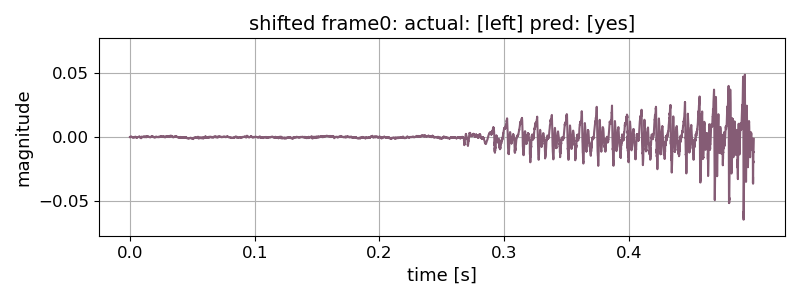
\includegraphics[width=0.48\textwidth]{./5_exp/figs/exp_details_tb_shift_left_frame0.png}}
    \quad
    \subfigure[frame shift 30]{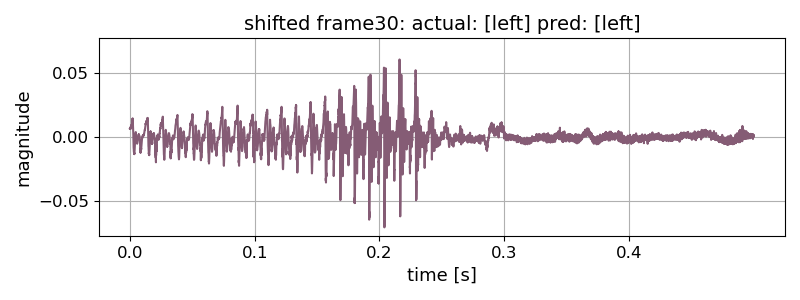
\includegraphics[width=0.48\textwidth]{./5_exp/figs/exp_details_tb_shift_left_frame30.png}}
    \subfigure[frame shift 59]{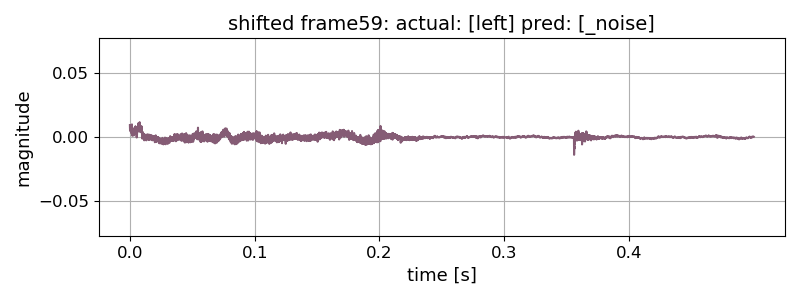
\includegraphics[width=0.48\textwidth]{./5_exp/figs/exp_details_tb_shift_left_frame59.png}}
  \caption{Shifting a self recorded example of the label \enquote{left} with certain amounts of frame shifts. The classification results are provided in the title annotations.}
  \label{fig:exp_details_tb_shift_left}
\end{figure}
\FloatBarrier
\noindent
The figures in this section present a correct classification with a colored pixel and an incorrect with a white one.
\rfig{exp_details_tb_shift} provides one example of a shift invariance test.
\begin{figure}[!ht]
  \centering
    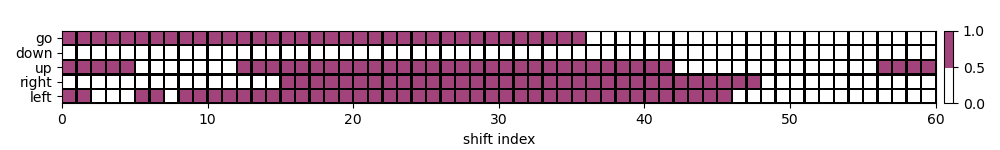
\includegraphics[width=0.65\textwidth]{./5_exp/figs/exp_fs_cepstral_tb_shift_conv-jim_mfcc12_norm0.png}
  \caption{Shift invariance test example selected from one of the trained models in the experiments.}
  \label{fig:exp_details_tb_shift}
\end{figure}
\FloatBarrier
\noindent
The purpose of the shift invariance test is not to achieve a full classification score upon each test example because this is hardly possible if not all of a keyword's information is captured within the shifted frame.
Conversely, the shift invariance test analyzes whether there are consecutive correct classifications within a certain region of shift indices.
Holes in this region are not a good indicator for the trained model.
If one example could not be classified at all, it does not necessarily imply that the trained model performs poorly but that this specific example is not recognized with this specific training instance of the model.
A well performing model usually has a wide region of correct classifications with no holes in it.


% --
% noise invariance

\subsubsection{Noise Invariance}
The classification of speech signals often requires noise invariance.
This is because a significant amount of noise added, for instance, through the use of poor microphones or recording set-ups, might disturb the classification accuracy.
To construct a test upon noise invariance, AWGN is added to the test signal $\bm{x} \in \R^n$ by
\begin{equation}
  \bm{\tilde{x}} = \bm{x} + \bm{v}, \quad \bm{v} \sim \mathcal{N}(\mu, \sigma),
\end{equation}
where $\bm{v} \in \R^n$ is the additive noise sampled from the normal distribution $\mathcal{N}(\mu, \sigma)$ with mean $\mu = 0$ and standard deviation $\sigma$.
The AWGN is parametrized through the standard deviation $\sigma$ to create a certain Signal to Noise Ratio (SNR), denoted as $S$.
Rewriting the formula of the SNR, the standard deviation can be obtained by
\begin{equation}
  \sigma = \sqrt{\frac{\frac{1}{n}\bm{x}^T \bm{x}}{10^{\frac{S}{10}}}}
\end{equation}
for requested SNR values $S$ in decibel (dB).
A SNR level of zero means that there is equal energy of the added noise $\bm{v}$ and the test signal $\bm{x}$, therefore, the resulting signal is already strong disturbed with noise.
\rfig{exp_details_tb_noise_left} provides an example of the noise invariance test with a low, middle, and high SNR value.
\begin{figure}[!ht]
  \centering
    \subfigure[\SI{16}{\dB}]{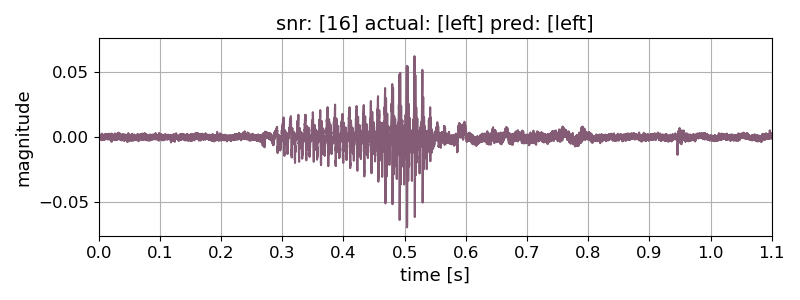
\includegraphics[width=0.48\textwidth]{./5_exp/figs/exp_details_tb_noise_left_snr16.png}}
    \quad
    \subfigure[\SI{0}{\dB}]{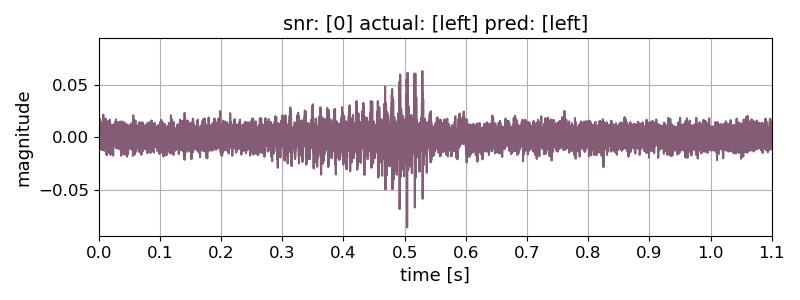
\includegraphics[width=0.48\textwidth]{./5_exp/figs/exp_details_tb_noise_left_snr0.png}}
    \subfigure[\SI{-16}{\dB}]{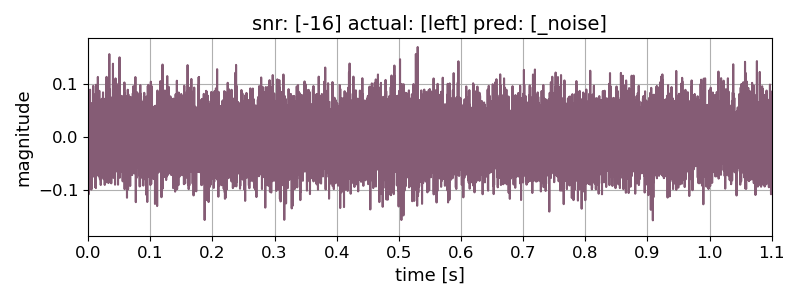
\includegraphics[width=0.48\textwidth]{./5_exp/figs/exp_details_tb_noise_left_snr-16.png}}
  \caption{Adding noise to a self recorded example of \enquote{left} with certain SNR values. The classification results are provided in the title annotations.}
  \label{fig:exp_details_tb_noise_left}
\end{figure}
\FloatBarrier
\noindent
The plots for the noise invariance test indicate the added noise through the SNR value on the x-axis.
\rfig{exp_details_tb_noise} shows an example of a noise invariance test.
\begin{figure}[!ht]
  \centering
    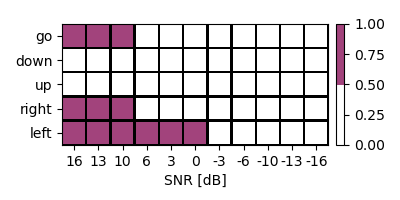
\includegraphics[width=0.35\textwidth]{./5_exp/figs/exp_fs_cepstral_tb_noise_conv-jim_mfcc12_norm0.png}
  \caption{Noise invariance test example selected from the trained models in the experiments.}
  \label{fig:exp_details_tb_noise}
\end{figure}
\FloatBarrier
\noindent
The same criteria, as described in the shift invariance, also applies to the noise invariance, where the region of consecutive correct classifications should start from low noise levels to high noise levels.

% experiments
% --
% feature selection

\section{Experiments on MFCC Feature Selection}\label{sec:exp_fs}
Feature selection is a very important step prior to neural network training.
A reduction of input features always means a reduction of computations, hence it is a crucial point to evaluate for finding energy efficient models.
Unfortunately it is not always clear which feature are contributing to good classification scores and which do not or even worsen them.
In this section only MFCCs and their enhancements, as described in \rsec{signal_mfcc}, are the focus in the experiments.
A feature selection for raw audio samples, such as used in the Wavenet architecture, would not make any sense because each sample is a feature itself.
Another important aspect in the feature selection experiments is the evaluation of the proposed frame-based normalization \req{signal_mfcc_norm} originally intended to improve the visualization of MFCCs and making the Generator network of GANs easier and faster to train.
However, frame-based normalization might be critical because this normalization applies only on the frame (time) dimension and disregards the frequency dimension.

Two experiments perform on the MFCC feature selection and evaluates:
\begin{enumerate}
    \item The impact on the amount of cepstral coefficients and
    \item the impact on the enhancements of MFCCs.
\end{enumerate}
For saving training time and computations, those experiments were done on a smaller training set than the whole speech commands dataset, described in \rsec{exp_dataset_speech_cmd}, by using 500 samples of each one of the L12 labels.
The filter bands of the MFCCs were fixed to a total number of 32 bands for all experiments.
Five consecutive training instances perform the training of one set of selected parameters on the same model to create better statistics for the evaluation scores.
The statistics present a mean value and the standard deviation (square root of the variance) of the accuracy scores from all training instances.
The experiments do not apply any early stopping mechanism and therefore use the model parameters from the last epoch for evaluation.
Note that the experiments in this sections are not meant for comparison to the benchmark networks, as described in \rsec{prev_kws_benchmark}, because not the whole dataset was used.


% --
% cepstral

\subsection{Impact on the Amount of Cepstral Coefficients}
The experiment on the impact of the amount of cepstral coefficients evaluates the accuracies of different neural network models using a number of either 12 or 32 cepstral coefficients from the extracted MFCCs.
Note that a number of 12 coefficients with enhancements is commonly applied in many papers.
The experiments were performed once with and once without frame-based normalization to observe its impact on the classification accuracy as well.
Further, the trained models were evaluated regarding their noise and shift invariance, as described in \rsec{exp_details_tb}.
The experiment uses the standard set of training hyperparameters, as listed in \rtab{exp_details_params_train}.
\rtab{exp_fs_cepstral_l12} shows the results of the experiment with 2000 training epochs performed on all three CNN models.
Note that the normalization is active if the table lists \enquote{1} in the \enquote{Norm.} column, otherwise the normalization is not applied and indicated with \enquote{0}.
\begin{table}[ht!]
\begin{center}
\caption{Experiment on the impact of the amount of cepstral coefficient of MFCC features with additional frame based normalization evaluation.}
\begin{tabular}{ M{3cm}  M{2cm}  M{2cm}  M{2.5cm}  M{2.5cm} }
\toprule
\textbf{arch} & \textbf{mfcc} & \textbf{norm} & \textbf{acc test} & \textbf{acc my} \\
\midrule
conv-trad & mfcc32-12 & 0 & $81.73 \pm 1.58$ & $80.80 \pm 5.88$ \\
conv-trad & mfcc32-12 & 1 & $75.97 \pm 1.15$ & $90.40 \pm 4.80$ \\
conv-trad & mfcc32-32 & 0 & $80.90 \pm 0.81$ & $81.60 \pm 7.84$ \\
conv-trad & mfcc32-32 & 1 & $74.93 \pm 1.09$ & $88.80 \pm 5.31$ \\
\midrule
conv-fstride & mfcc32-12 & 0 & $74.03 \pm 0.87$ & $73.60 \pm 8.62$ \\
conv-fstride & mfcc32-12 & 1 & $66.33 \pm 1.29$ & $79.20 \pm 6.40$ \\
conv-fstride & mfcc32-32 & 0 & $72.07 \pm 2.24$ & $72.80 \pm 8.54$ \\
conv-fstride & mfcc32-32 & 1 & $63.63 \pm 1.15$ & $91.20 \pm 1.60$ \\
\midrule
conv-jim & mfcc32-12 & 0 & $78.73 \pm 1.55$ & $76.00 \pm 6.69$ \\
conv-jim & mfcc32-12 & 1 & $71.77 \pm 1.77$ & $73.60 \pm 5.43$ \\
conv-jim & mfcc32-32 & 0 & $76.43 \pm 1.52$ & $83.20 \pm 2.99$ \\
conv-jim & mfcc32-32 & 1 & $65.73 \pm 1.94$ & $67.20 \pm 6.88$ \\
\bottomrule
\label{tab:exp_fs_cepstral_l12}
\end{tabular}
\end{center}
\end{table}
\FloatBarrier
\noindent
\rfig{exp_fs_cepstral_acc} shows the accuracies on the validation set of the best performing training instances for each model where the accuracies are smoothed by a striding average filter with a length of 10 epochs for better visualization.
\begin{figure}[!ht]
  \centering
  \subfigure[conv-trad]{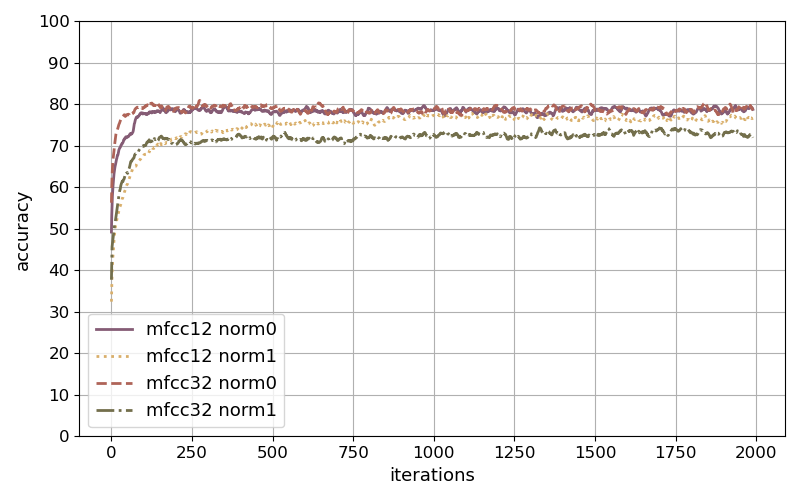
\includegraphics[width=0.45\textwidth]{./5_exp/figs/exp_fs_cepstral_acc_conv-trad.png}}
  \subfigure[conv-fstride]{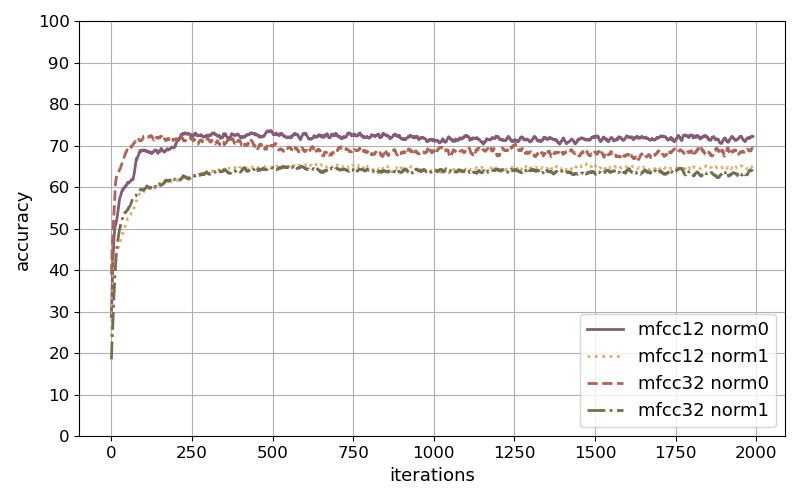
\includegraphics[width=0.45\textwidth]{./5_exp/figs/exp_fs_cepstral_acc_conv-fstride.png}}
  \subfigure[conv-jim]{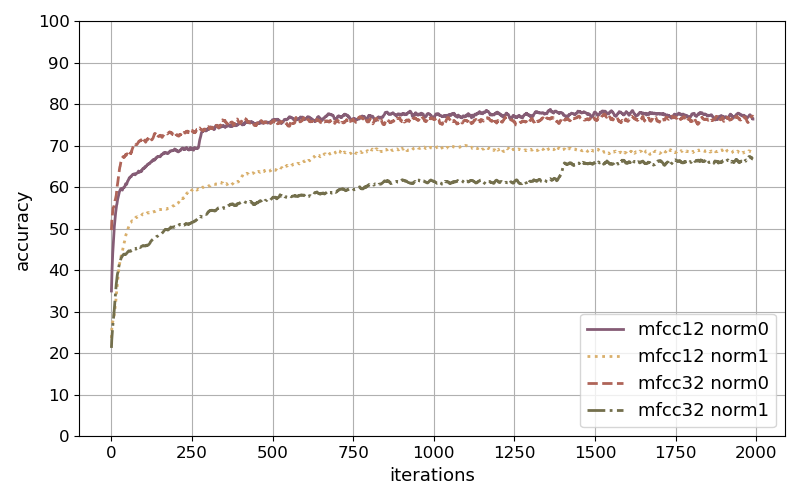
\includegraphics[width=0.45\textwidth]{./5_exp/figs/exp_fs_cepstral_acc_conv-jim.png}}
  \caption{Accuracies on the validation set of all three CNN models of their best training instance with different amounts of cepstral coefficients and with and without frame-based normalization. Applied smoothing with a 10 epoch average filter.}
  \label{fig:exp_fs_cepstral_acc}
\end{figure}
\FloatBarrier
\noindent
From the provided results, it can be observed that the usage of 32 cepstral coefficients does not improve the accuracies compared to the 12 coefficients.
Also the overfitting effects are more prominent when 32 coefficients are applied.
Moreover, they show that frame-based normalization usually achieves a lower accuracy and requires more epochs until convergence is reached.

In the following, the shift and noise invariance of each model is evaluated.
The noise and shift invariance of the \texttt{conv-trad} model is shown in \rfig{exp_fs_cepstral_tb_noise_conv-trad} and \rfig{exp_fs_cepstral_tb_shift_conv-trad} respectively.
\begin{figure}[!ht]
  \centering
  \subfigure[mfcc12, norm0]{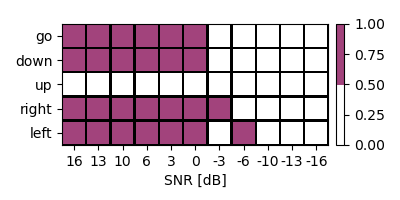
\includegraphics[width=0.35\textwidth]{./5_exp/figs/exp_fs_cepstral_tb_noise_conv-trad_mfcc12_norm0.png}}
  \subfigure[mfcc12, norm1]{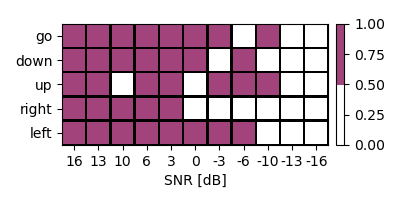
\includegraphics[width=0.35\textwidth]{./5_exp/figs/exp_fs_cepstral_tb_noise_conv-trad_mfcc12_norm1.png}}
  \subfigure[mfcc32, norm0]{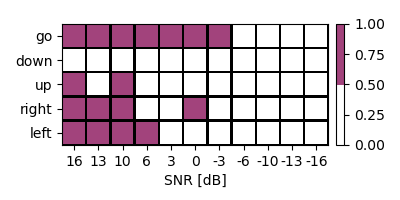
\includegraphics[width=0.35\textwidth]{./5_exp/figs/exp_fs_cepstral_tb_noise_conv-trad_mfcc32_norm0.png}}
  \subfigure[mfcc32, norm1]{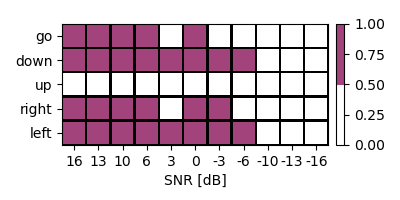
\includegraphics[width=0.35\textwidth]{./5_exp/figs/exp_fs_cepstral_tb_noise_conv-trad_mfcc32_norm1.png}}
  \caption{Noise invariance of the \texttt{conv-trad} model with different amounts of cepstral coefficients and with and without frame-based normalization.}
  \label{fig:exp_fs_cepstral_tb_noise_conv-trad}
\end{figure}
\FloatBarrier
\noindent
\begin{figure}[!ht]
  \centering
  \subfigure[mfcc12, norm0]{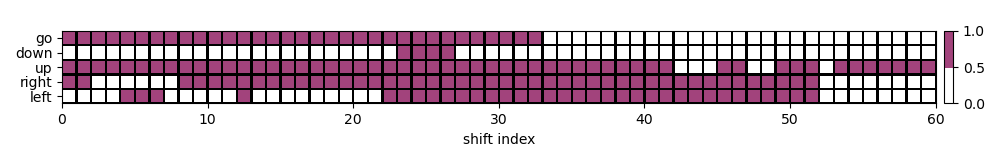
\includegraphics[width=0.45\textwidth]{./5_exp/figs/exp_fs_cepstral_tb_shift_conv-trad_mfcc12_norm0.png}}
  \subfigure[mfcc12, norm1]{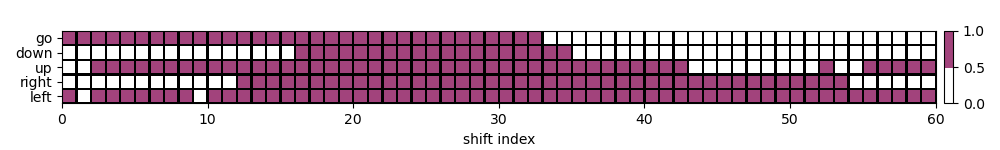
\includegraphics[width=0.45\textwidth]{./5_exp/figs/exp_fs_cepstral_tb_shift_conv-trad_mfcc12_norm1.png}}
  \subfigure[mfcc32, norm0]{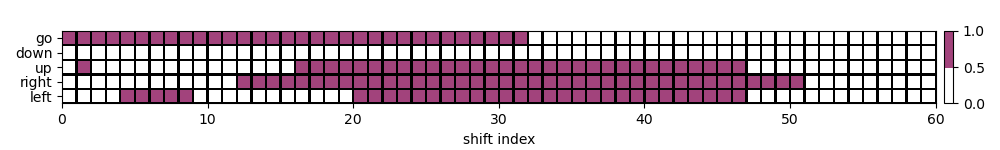
\includegraphics[width=0.45\textwidth]{./5_exp/figs/exp_fs_cepstral_tb_shift_conv-trad_mfcc32_norm0.png}}
  \subfigure[mfcc32, norm1]{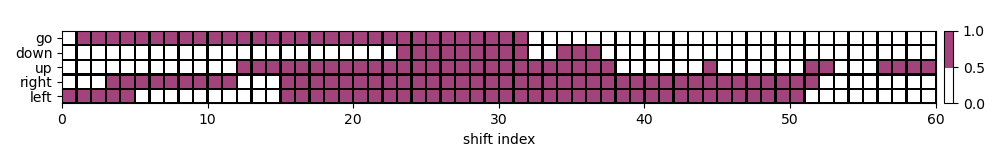
\includegraphics[width=0.45\textwidth]{./5_exp/figs/exp_fs_cepstral_tb_shift_conv-trad_mfcc32_norm1.png}}
  \caption{Shift invariance of the \texttt{conv-trad} model with different amounts of cepstral coefficients and with and without frame-based normalization.}
  \label{fig:exp_fs_cepstral_tb_shift_conv-trad}
\end{figure}
\FloatBarrier
\noindent
The noise and shift invariance of the \texttt{conv-fstride} model is shown in \rfig{exp_fs_cepstral_tb_noise_conv-fstride} and \rfig{exp_fs_cepstral_tb_shift_conv-fstride} respectively.
\begin{figure}[!ht]
  \centering
  \subfigure[mfcc12, norm0]{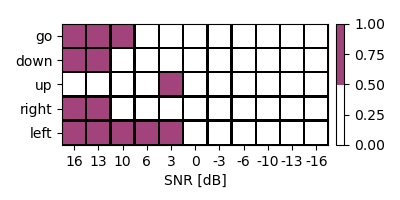
\includegraphics[width=0.35\textwidth]{./5_exp/figs/exp_fs_cepstral_tb_noise_conv-fstride_mfcc12_norm0.png}}
  \subfigure[mfcc12, norm1]{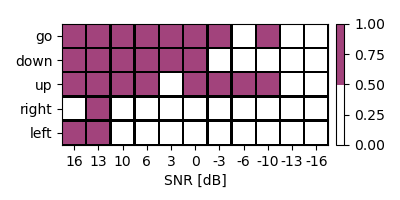
\includegraphics[width=0.35\textwidth]{./5_exp/figs/exp_fs_cepstral_tb_noise_conv-fstride_mfcc12_norm1.png}}
  \subfigure[mfcc32, norm0]{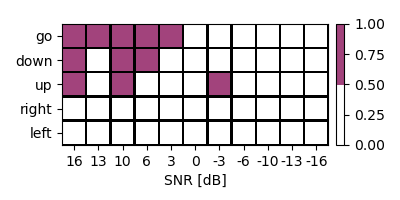
\includegraphics[width=0.35\textwidth]{./5_exp/figs/exp_fs_cepstral_tb_noise_conv-fstride_mfcc32_norm0.png}}
  \subfigure[mfcc32, norm1]{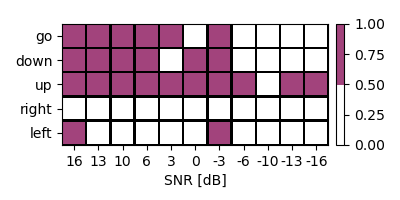
\includegraphics[width=0.35\textwidth]{./5_exp/figs/exp_fs_cepstral_tb_noise_conv-fstride_mfcc32_norm1.png}}
  \caption{Noise invariance of the \texttt{conv-fstride} model with different amounts of cepstral coefficients and with and without frame-based normalization.}
  \label{fig:exp_fs_cepstral_tb_noise_conv-fstride}
\end{figure}
\FloatBarrier
\noindent
\begin{figure}[!ht]
  \centering
  \subfigure[mfcc12, norm0]{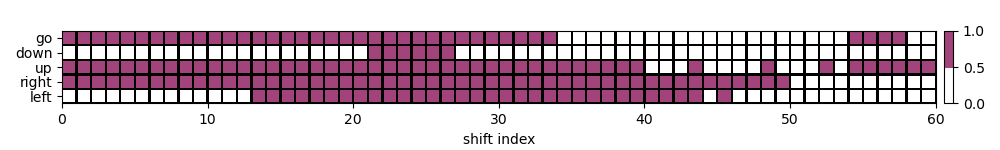
\includegraphics[width=0.45\textwidth]{./5_exp/figs/exp_fs_cepstral_tb_shift_conv-fstride_mfcc12_norm0.png}}
  \subfigure[mfcc12, norm1]{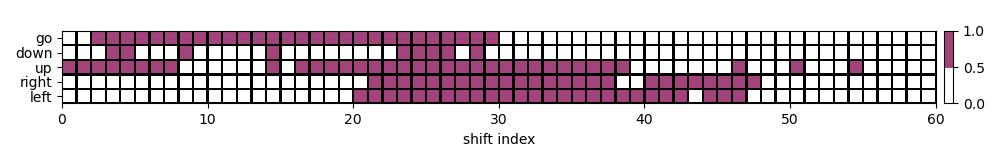
\includegraphics[width=0.45\textwidth]{./5_exp/figs/exp_fs_cepstral_tb_shift_conv-fstride_mfcc12_norm1.png}}
  \subfigure[mfcc32, norm0]{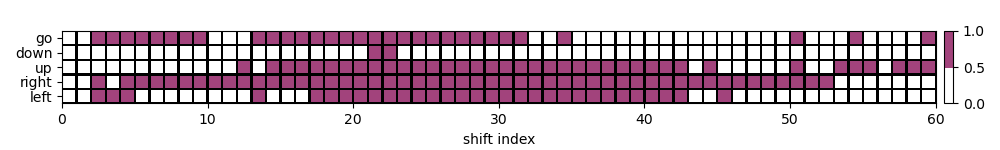
\includegraphics[width=0.45\textwidth]{./5_exp/figs/exp_fs_cepstral_tb_shift_conv-fstride_mfcc32_norm0.png}}
  \subfigure[mfcc32, norm1]{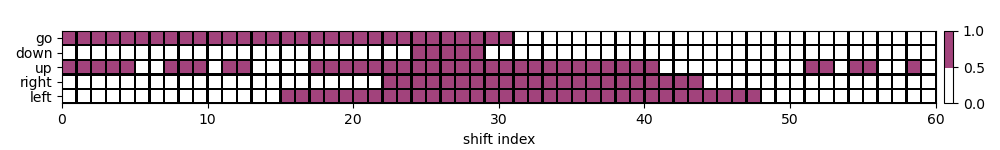
\includegraphics[width=0.45\textwidth]{./5_exp/figs/exp_fs_cepstral_tb_shift_conv-fstride_mfcc32_norm1.png}}
  \caption{Shift invariance of the \texttt{conv-fstride} model with different amounts of cepstral coefficients and with and without frame-based normalization.}
  \label{fig:exp_fs_cepstral_tb_shift_conv-fstride}
\end{figure}
\FloatBarrier
\noindent
The noise and shift invariance of the \texttt{conv-jim} model is shown in \rfig{exp_fs_cepstral_tb_noise_conv-jim} and \rfig{exp_fs_cepstral_tb_shift_conv-jim} respectively.
\begin{figure}[!ht]
  \centering
  \subfigure[mfcc12, norm0]{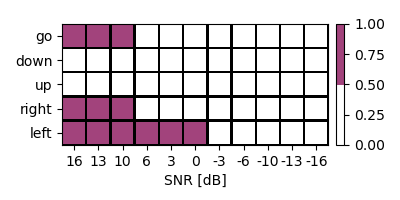
\includegraphics[width=0.35\textwidth]{./5_exp/figs/exp_fs_cepstral_tb_noise_conv-jim_mfcc12_norm0.png}}
  \subfigure[mfcc12, norm1]{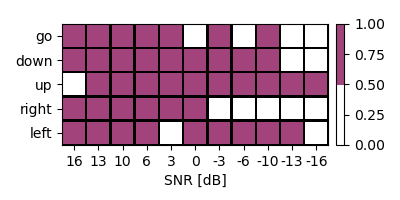
\includegraphics[width=0.35\textwidth]{./5_exp/figs/exp_fs_cepstral_tb_noise_conv-jim_mfcc12_norm1.png}}
  \subfigure[mfcc32, norm0]{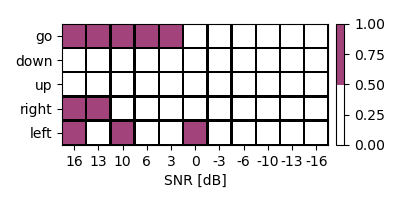
\includegraphics[width=0.35\textwidth]{./5_exp/figs/exp_fs_cepstral_tb_noise_conv-jim_mfcc32_norm0.png}}
  \subfigure[mfcc32, norm1]{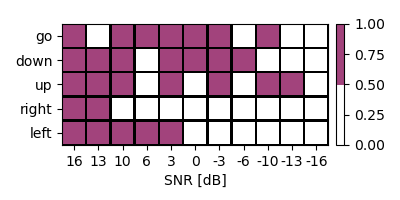
\includegraphics[width=0.35\textwidth]{./5_exp/figs/exp_fs_cepstral_tb_noise_conv-jim_mfcc32_norm1.png}}
  \caption{Noise invariance of the \texttt{conv-jim} model with different amounts of cepstral coefficients and with and without frame-based normalization.}
  \label{fig:exp_fs_cepstral_tb_noise_conv-jim}
\end{figure}
\FloatBarrier
\noindent
\begin{figure}[!ht]
  \centering
  \subfigure[mfcc12, norm0]{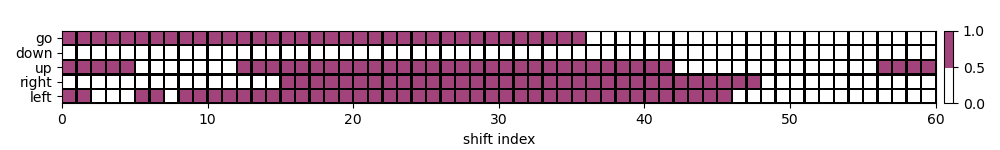
\includegraphics[width=0.45\textwidth]{./5_exp/figs/exp_fs_cepstral_tb_shift_conv-jim_mfcc12_norm0.png}}
  \subfigure[mfcc12, norm1]{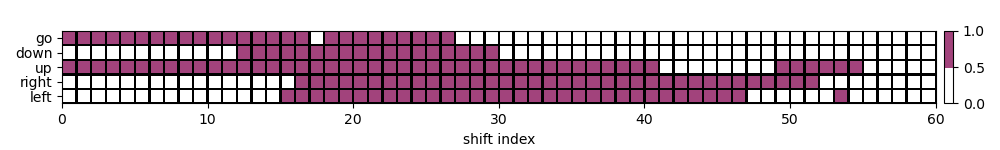
\includegraphics[width=0.45\textwidth]{./5_exp/figs/exp_fs_cepstral_tb_shift_conv-jim_mfcc12_norm1.png}}
  \subfigure[mfcc32, norm0]{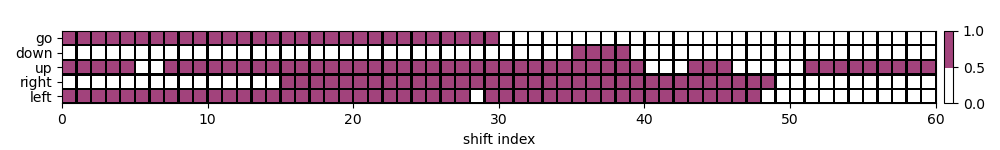
\includegraphics[width=0.45\textwidth]{./5_exp/figs/exp_fs_cepstral_tb_shift_conv-jim_mfcc32_norm0.png}}
  \subfigure[mfcc32, norm1]{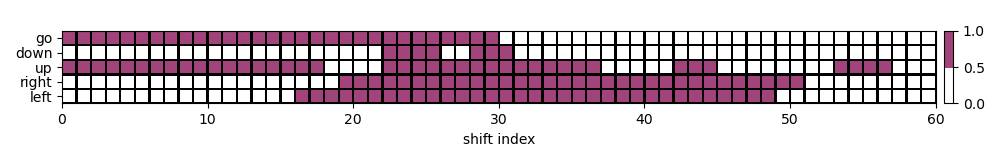
\includegraphics[width=0.45\textwidth]{./5_exp/figs/exp_fs_cepstral_tb_shift_conv-jim_mfcc32_norm1.png}}
  \caption{Shift invariance of the \texttt{conv-jim} model with different amounts of cepstral coefficients and with and without frame-based normalization.}
  \label{fig:exp_fs_cepstral_tb_shift_conv-jim}
\end{figure}
\FloatBarrier
\noindent
While the results of the invariance tests do not allow a general conclusion, following patterns can be observed regardless:
The frame-based normalization does certainly increase the invariance in noise, which is logical because the model has to focus more on learning patterns of the individual key words and is less prone to overfitting.
The \texttt{conv-fstride} model does unexpectedly well upon the shift invariance test, even though its strides perform merely on the frequency axis.
Although it usually does not achieve that good shift invariance results compared to the other models and often holes appear in the classification with the shift invariance test.
The \texttt{conv-trad} model performs best on all tests yet also requires a higher computational footprint so that the preferred model is the \texttt{conv-jim} model by providing a good trade-off between computational footprint and classification results.
The usage of 32 MFCC coefficients does not improve the invariance against shift or noise and very often worsens the results.


% --
% enhancements

\subsection{Impact on the Enhancements of MFCCs}\label{sec:exp_fs_mfcc}
In this experiment the cepstral coefficients were selected to 12 and enhanced with deltas, double deltas and energy vectors, as described in \rsec{signal_mfcc_enhancement}.
\rtab{exp_fs_mfcc_l12} lists the results of the experiments with applied frame-based normalization, 2000 training epochs and the standard hyperparameters for CNN models.
Note that a \enquote{1} in the columns for the enhancements means that a specific enhancement is included, otherwise it is denoted as \enquote{0}. 
\begin{table}[ht!]
\small
\begin{center}
\caption{Experiment on the impact of feature enhancement of cepstral coefficients (c), deltas (d), double deltas (dd) and energy vectors (e) performed on the \texttt{conv-jim} model with frame-based normalization}
\begin{tabular}{ M{1cm}  M{1cm}  M{1cm}  M{1cm}  M{2.5cm}  M{2.5cm} }
\toprule
\textbf{c} & \textbf{d} & \textbf{dd} & \textbf{e} & \textbf{acc test} & \textbf{acc my} \\
\midrule
0 & 0 & 1 & 0 & $37.40 \pm 2.17$ & $34.40 \pm 11.20$ \\
0 & 0 & 1 & 1 & $46.63 \pm 2.87$ & $36.80 \pm 7.76$ \\
0 & 1 & 0 & 0 & $58.57 \pm 2.06$ & $64.80 \pm 4.66$ \\
0 & 1 & 0 & 1 & $62.00 \pm 1.82$ & $75.20 \pm 11.14$ \\
0 & 1 & 1 & 0 & $59.03 \pm 1.77$ & $56.00 \pm 9.47$ \\
0 & 1 & 1 & 1 & $61.60 \pm 2.28$ & $62.40 \pm 6.97$ \\
1 & 0 & 0 & 0 & $72.00 \pm 1.46$ & $85.60 \pm 1.96$ \\
1 & 0 & 0 & 1 & $72.83 \pm 1.22$ & $80.00 \pm 4.38$ \\
1 & 0 & 1 & 0 & $70.63 \pm 2.13$ & $84.00 \pm 8.76$ \\
1 & 0 & 1 & 1 & $72.36 \pm 2.27$ & $80.00 \pm 4.38$ \\
1 & 1 & 0 & 0 & $72.80 \pm 2.90$ & $88.80 \pm 6.88$ \\
1 & 1 & 0 & 1 & $75.30 \pm 1.38$ & $92.00 \pm 2.53$ \\
1 & 1 & 1 & 0 & $73.43 \pm 2.05$ & $84.80 \pm 5.88$ \\
1 & 1 & 1 & 1 & $73.73 \pm 1.66$ & $83.20 \pm 6.88$ \\
\bottomrule
\label{tab:exp_fs_mfcc_l12}
\end{tabular}
\end{center}
\vspace{-4mm}
\end{table}
\FloatBarrier
\noindent
The best two feature enhancements were the full MFCC-39 features (c1d1d1e1) and the (c1d1d0e1) features without double deltas.
Those were used for examining the accuracy on the validation set during training shown in \rfig{exp_fs_mfcc_tb_acc_conv-jim} and the noise and shift invariance in \rfig{exp_fs_mfcc_tb_noise_conv-jim} and \rfig{exp_fs_mfcc_tb_shift_conv-jim}.
\begin{figure}[!ht]
  \centering
  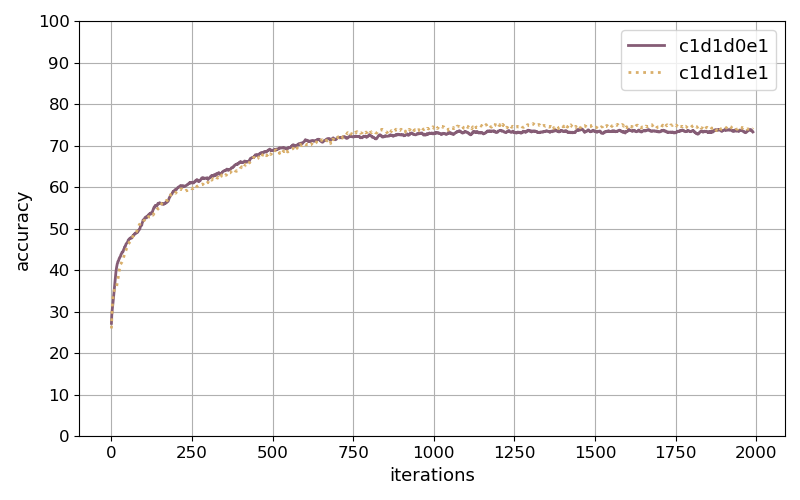
\includegraphics[width=0.45\textwidth]{./5_exp/figs/exp_fs_mfcc_acc_conv-jim.png}
  \caption{Accuracies of the \texttt{conv-jim} model with different feature enhancements and frame-based normalization.}
  \label{fig:exp_fs_mfcc_tb_acc_conv-jim}
\end{figure}
\FloatBarrier
\noindent
\begin{figure}[!ht]
  \centering
  \subfigure[c1d1d1e1]{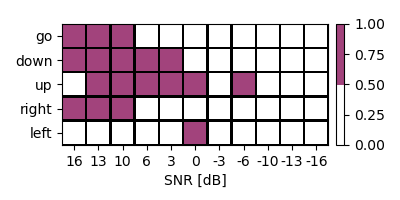
\includegraphics[width=0.35\textwidth]{./5_exp/figs/exp_fs_mfcc_tb_noise_conv-jim_c1d1d1e1.png}}
  \subfigure[c1d1d0e1]{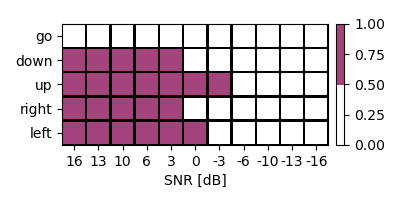
\includegraphics[width=0.35\textwidth]{./5_exp/figs/exp_fs_mfcc_tb_noise_conv-jim_c1d1d0e1.png}}
  \caption{Noise invariance of the \texttt{conv-jim} model with different feature enhancements and frame-based normalization.}
  \label{fig:exp_fs_mfcc_tb_noise_conv-jim}
\end{figure}
\FloatBarrier
\noindent
\begin{figure}[!ht]
  \centering
  \subfigure[c1d1d1e1]{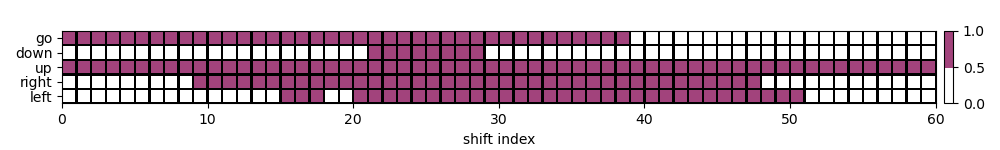
\includegraphics[width=0.45\textwidth]{./5_exp/figs/exp_fs_mfcc_tb_shift_conv-jim_c1d1d1e1.png}}
  \subfigure[c1d1d0e1]{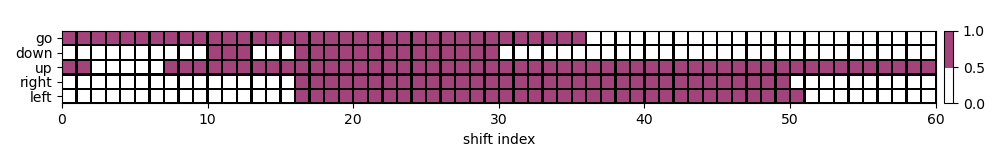
\includegraphics[width=0.45\textwidth]{./5_exp/figs/exp_fs_mfcc_tb_shift_conv-jim_c1d1d0e1.png}}
  \caption{Shift invariance of the \texttt{conv-jim} model with different feature enhancements and frame-based normalization.}
  \label{fig:exp_fs_mfcc_tb_shift_conv-jim}
\end{figure}
\FloatBarrier
\noindent
The experiments show that the enhancements of the MFCC features can improve the classification results significantly yet also increases the amount of computations for each model.
% --
% adversarial training

\section{Experiments on Adversarial Pre-Training}\label{sec:exp_adv}
Adversarial pre-training, as already described in detail in \rsec{nn_adv}, is the transfer of learned weights obtained from an adversarial training between a Generator and a Discriminator network from a GAN.
The neural network architecture used for adversarial pre-training is the \texttt{conv-jim} model, as described in \rsec{nn_arch_cnn}.
The \texttt{conv-jim} model initializes its weights from pre-trained weights of its GAN versions, namely the \texttt{adv-d-jim} and \texttt{adv-g-jim}, which are described in \rsec{nn_arch_adv}.
Note that frame-based normalization was applied, which made the training of GANs considerably faster and the weights from G applicable.
Both adversarial pre-training methods, the adversarial label and dual train, were evaluated.

Note that the experiments in this section, like in the previous section, are not meant for comparison to the benchmark networks because of an usage of 500 examples per class instead of the whole dataset.
Also no overfitting mechanism was applied in this experiments.


% --
% label train

\subsection{Impact of Adversarial Label Train}\label{sec:exp_adv_label}
The adversarial label training experiments on the \texttt{conv-jim} architecture with obtained weights from either \texttt{adv-g-jim} or \texttt{adv-d-jim} are presented in \rtab{exp_adv_label_l12}.
\begin{table}[ht!]
\small
\begin{center}
\caption{Experiment with adversarial label pre-training, using either Generator \enquote{g} or Discriminator \enquote{d} weights.}
\begin{tabular}{ M{2cm}  M{2cm}  M{2.5cm}  M{2.5cm} }
\toprule
\textbf{adv iterations} & \textbf{adv model} & \textbf{acc test} & \textbf{acc my} \\
\midrule
100 & g & $75.80 \pm 2.17$ & $85.60 \pm 4.08$ \\
100 & d & $73.57 \pm 1.59$ & $83.20 \pm 6.40$ \\
1000 & g & $74.83 \pm 2.15$ & $85.60 \pm 4.08$ \\
1000 & d & $73.36 \pm 0.86$ & $84.00 \pm 5.06$ \\
\bottomrule
\label{tab:exp_adv_label_l12}
\end{tabular}
\end{center}
\vspace{-4mm}
\end{table}
\FloatBarrier
\noindent
It can be observed that the weights from the Generator network achieves better performances than the weights from the Discriminator network.
\rfig{exp_adv_label_acc_conv-jim} shows the best performing models in one single accuracy plot.
\begin{figure}[!ht]
  \centering
  \includegraphics[width=0.48\textwidth]{./5_exp/figs/exp_adv_label_acc_conv-jim.png}
  \caption{Accuracies of the \texttt{conv-jim} model with different adversarial label training and frame-based normalization. The results were smoothed with a 10 epoch average filter.}
  \label{fig:exp_adv_label_acc_conv-jim}
\end{figure}
\FloatBarrier
\noindent
The noise and shift invariance tests are provided in \rfig{exp_adv_label_tb_noise_conv-jim} and \rfig{exp_adv_label_tb_shift_conv-jim}, respectively.
\begin{figure}[!ht]
  \centering
  \subfigure[D]{\includegraphics[width=0.35\textwidth]{./5_exp/figs/exp_adv_label_tb_noise_conv-jim_d-100.png}}
  \qquad
  \subfigure[G]{\includegraphics[width=0.35\textwidth]{./5_exp/figs/exp_adv_label_tb_noise_conv-jim_g-100.png}}
  \caption{Noise invariance of the \texttt{conv-jim} model with adversarial label training of 100 epochs and using either the Generator or Discriminator weights.}
  \label{fig:exp_adv_label_tb_noise_conv-jim}
\end{figure}
\FloatBarrier
\noindent
\begin{figure}[!ht]
  \centering
  \subfigure[D]{\includegraphics[width=0.48\textwidth]{./5_exp/figs/exp_adv_label_tb_shift_conv-jim_d-100.png}}
  \quad
  \subfigure[G]{\includegraphics[width=0.48\textwidth]{./5_exp/figs/exp_adv_label_tb_shift_conv-jim_g-100.png}}
  \caption{Shift invariance of the \texttt{conv-jim} model with adversarial label training of 100 epochs and using either the Generator or Discriminator weights.}
  \label{fig:exp_adv_label_tb_shift_conv-jim}
\end{figure}
\FloatBarrier
\noindent
In many experiments the noise and shift invariance show improvements when adversarial pre-training is applied. 


% --
% adv dual train

\subsection{Impact of Adversarial Dual Train}
The adversarial dual training experiments were similar to the adversarial label train ones but without choosing subsets of labels and simply using the same convolutional layer structure for the Generator and Discriminator model like the CNN.
The experiments are presented in \rtab{exp_adv_dual_l12}.
\begin{table}[ht!]
\small
\begin{center}
\caption{Experiment with adversarial dual pre-training, using either Generator or Discriminator weights.}
\begin{tabular}{ M{2cm}  M{2cm}  M{2.5cm}  M{2.5cm} }
\toprule
\multicolumn{2}{c}{\textbf{Adversarial}} & \multicolumn{2}{c}{\textbf{Accuracy [\%]}}\\
Epochs & Model & Test set & My dataset\\
\midrule
100 & G & $73.53 \pm 1.75$ & $79.20 \pm 7.33$ \\
100 & D & $69.03 \pm 6.53$ & $72.80 \pm 15.88$ \\
1000 & G & $73.53 \pm 1.53$ & $84.00 \pm 4.38$ \\
1000 & D & $72.57 \pm 1.05$ & $83.20 \pm 2.99$ \\
\bottomrule
\label{tab:exp_adv_dual_l12}
\end{tabular}
\end{center}
\vspace{-4mm}
\end{table}
\FloatBarrier
\noindent
The dual experiments achieved worse accuracies for the transfer of Discriminator weights compared to the initializing of the target model with random weights.
The Generator weights however, could increase the average accuracy by at least \SI{1}{\percent}.
The dual training is not further evaluated regarding noise and shift invariance because the adv-label training performed better.
% --
% wavenets

\section{Experiments on Wavenets}\label{exp_wavenet}
Very few experiments were performed on the Wavenet architecture because of its complex model structure and heavy computational footprint, as already mentioned in \rsec{nn_arch_wavenet}.
The Wavenet model requires a generous amount of time and energy consumption for very few training epochs.
Furthermore, the experiments showed poor results on the accuracy of classifying speech commands.
This architecture is therefore left for future research.
Nevertheless, this section presents the best performing Wavenet model on the KWS task.
The training details for this model were 500 examples per each one of the L12 labels, 100 epochs, a learning rate of $0.001$ for 10 epochs that changes aftwerwards to $0.0001$, and a batch size of 32.
\rfig{exp_wavenet_acc} shows the accuracy score for the training and \rfig{exp_wavenet_confusion} provides the confusion matrix on the test set.
However, the best achieved accuracy on the test set was merely \SI{38.83}{\percent}.
\begin{figure}[!ht]
  \centering
  \includegraphics[width=0.45\textwidth]{./5_exp/figs/exp_wavenet_acc.png}
  \caption{Accuracies on the validation set during the training of the Wavenet model with classification extension.}
  \label{fig:exp_wavenet_acc}
\end{figure}
\begin{figure}[!ht]
  \centering
  \includegraphics[width=0.45\textwidth]{./5_exp/figs/exp_wavenet_confusion_test.png}
  \caption{Confusion matrix on the test set evaluated on the trained Wavenet model.}
  \label{fig:exp_wavenet_confusion}
\end{figure}
\FloatBarrier
\noindent
% --
% Experiments on whole dataset

\section{Experiments on whole dataset}\label{sec:exp_final}
The final experiments were performed on the whole dataset with 3500 examples per labels and are therefore used for comparison to the benchmark models listed in \rsec{prev_kws_benchmark}.
All CNN architectures were evaluated with 12 MFCC coefficients and the application of either frame-based normalization or no normalization.
A single run with 2000 epochs was performed for all experiments to save computational effort.
The evaluation on the adversarial pre-training, as described in \rsec{exp_adv}, was done for the \texttt{conv-jim} model in a separate run.
\rtab{exp_final_l12} shows the results of the experiments.
\begin{table}[ht!]
\small
\begin{center}
\caption{Experiment on the whole dataset with 3500 examples per label, 12 MFCC coefficients and 2000 epochs.}
\begin{tabular}{ M{3cm}  M{1.5cm}  M{2.5cm}  M{2.5cm}  M{2.5cm} }
\toprule
\multirow{2}{*}{\centering\textbf{Model Name}} & \multirow{2}{*}{\centering\textbf{Norm.}} & \multirow{2}{*}{\centering\textbf{Pre-Train}} & \multicolumn{2}{c}{\textbf{Accuracy}}\\
& & & Test set & My dataset\\
\midrule
conv-trad & 0 & - & $84.52$ & $92.00$ \\
conv-fstride & 0 & - & $79.76$ & $80.00$ \\
conv-jim & 0 & - & $87.14$ & $88.00$ \\
\midrule
conv-trad & 1 & - & $83.79$ & $88.00$ \\
conv-fstride & 1 & - & $78.71$ & $92.00$ \\
conv-jim & 1 & - & $82.36$ & $88.00$ \\
\midrule
conv-jim & 1 & adv-label-100 & $84.62$ & $92.00$ \\
\bottomrule
\label{tab:exp_final_l12}
\end{tabular}
\end{center}
\vspace{-4mm}
\end{table}
\FloatBarrier
\noindent
Note that there are some overfitting effects happening, especially showing up in the not normalized training of the \texttt{conv-trad} model in \rfig{exp_final_loss_conv-trad}.
It is therefore useful to use an early stopping technique for better generalization that obtains the model parameters at the best performing training epoch evaluated on the validation set.
\begin{figure}[!ht]
  \centering
  \subfigure[norm0]{\includegraphics[width=0.45\textwidth]{./5_exp/figs/exp_final_loss_norm0_conv-trad.png}}
  \subfigure[norm1]{\includegraphics[width=0.45\textwidth]{./5_exp/figs/exp_final_loss_norm1_conv-trad.png}}
  \caption{Training loss of the \texttt{conv-trad} model showing overfitting effects on the whole dataset.}
  \label{fig:exp_final_loss_conv-trad}
\end{figure}
\FloatBarrier
\noindent
The training of models with frame-based normalization usually had less problems with overfitting compared to when no normalization was applied.
The accuracy performance on the validation set of all models with and without frame-based normalization is shown in \rfig{exp_final_acc}.
\begin{figure}[!ht]
  \centering
  \subfigure[norm0]{\includegraphics[width=0.45\textwidth]{./5_exp/figs/exp_final_acc_norm0.png}}
  \subfigure[norm1]{\includegraphics[width=0.45\textwidth]{./5_exp/figs/exp_final_acc_norm1.png}}
  \caption{Training accuracies of all models with and without frame-based normalization performed on the whole dataset, averaged over 10 epochs for better visualization.}
  \label{fig:exp_final_acc}
\end{figure}
\FloatBarrier
\noindent
Note that the accuracy scores had been smoothed over the epochs and that usually some spikes in performances are present and should be avoided.
Therefore it is strongly recommended to use early stopping.
For instance, the \texttt{conv-trad} without frame-based normalization could have got a better score if early stopping would have been used.

There is a large gap between the evaluated models and the benchmark models in \rsec{prev_kws_benchmark}.
With \SI{84.62}{\percent} the \texttt{conv-jim} model with adversarial pre-training performs about \SI{10}{\percent} worse than the benchmark model (DS-CNN-S \cite{Zhang2017}) with \SI{94.4}{\percent}.
However it must be considered that the amount of operations for the \texttt{conv-jim} model are about 6 times less than the DS-CNN-S and that not the whole audio file of \SI{1}{\second} was processed, but a shorter time interval of \SI{500}{\milli\second}.
With this in mind, the results do not look that poorly.
To observe the problems in classification, a confusion matrix from the \texttt{conv-jim} model with adversarial label train on the Generator weights, is shown in \rfig{exp_final_confusion}.
\begin{figure}[!ht]
  \centering
  \includegraphics[width=0.45\textwidth]{./5_exp/figs/exp_final_confusion.png}
  \caption{Confusion matrix of the \texttt{conv-jim} model pre-trained with adversarial label train of 100 epochs using the Generator weights, and 2000 epochs of usual training, with frame-based normalization applied.}
  \label{fig:exp_final_confusion}
\end{figure}
\FloatBarrier
\noindent
From the confusion matrix it can be observed, that most classifications are done correctly and that misconceptions usually happens at similar words with the same used phonemes, like \enquote{go} and \enquote{no}.
The mixed labels also add more difficulty to the classification task and drags the scores down.

The weights of the first convolutional layers of the trained model weights are visualized in \rsec{appendix_weights}.
All in all the obtained scores should be sufficient for a video game application.